\documentclass[11pt]{article}

% Shared notes settings for Applied Machine Learning lectures (UPES).
% Keep this file free of \documentclass to allow reuse via \input.

\usepackage[utf8]{inputenc}
\usepackage[T1]{fontenc}
\usepackage{lmodern}          % scalable T1 fonts; without this pdflatex falls back
\input{glyphtounicode}        % to bitmapped EC Type 3 and the PDFs are neither
\pdfgentounicode=1            % searchable nor screen-reader friendly
\usepackage[a4paper,margin=1in]{geometry}
\usepackage{hyperref}
\usepackage{xurl}
\usepackage{booktabs}
\usepackage{amsmath}
\usepackage{amssymb}
\usepackage{listings}
\usepackage{xcolor}
\usepackage{enumitem}
\usepackage{parskip}

% Code listings (Python-oriented for this subject).
\lstset{
  language=Python,
  basicstyle=\ttfamily\small,
  keywordstyle=\color{blue},
  commentstyle=\color{gray},
  stringstyle=\color{teal},
  showstringspaces=false,
  columns=fullflexible,
  frame=single,
  framerule=0.2pt,
  breaklines=true
}

\setlist[itemize]{topsep=0.3em,itemsep=0.2em}
\setlist[enumerate]{topsep=0.3em,itemsep=0.2em}

% Simple per-section source line.
\newcommand{\notesources}[1]{\par\noindent{\small\color{gray}\textit{Sources:} \sloppy #1\par}}

% Unit-wise source strings for this subject (used by slides + notes).
% Path is relative to the lecture `latex/` folder (the compilation CWD).
\IfFileExists{../../../_shared/aml-sources.tex}{%
  % Source strings for Applied Machine Learning (CSAI2017P) — used by slides + notes.
% Prescribed texts and reference books are taken from the course syllabus.
% Support texts are the author-hosted open-access editions:
%   statlearning.com            (ISL with Python)
%   probml.github.io/pml-book   (Murphy, Probabilistic Machine Learning)
%   d2l.ai                      (Dive into Deep Learning)
%   mml-book.github.io          (Mathematics for Machine Learning)

\newcommand{\AMLRepoURL}{https://github.com/tali7c/Applied-Machine-Learning}

% --- prescribed -------------------------------------------------------------
\newcommand{\AMLPrescribed}{%
M\"uller and Guido, \textit{Introduction to Machine Learning with Python}, O'Reilly, 2016.;%
Bishop, \textit{Pattern Recognition and Machine Learning}, Springer, 2006.;%
Murphy, \textit{Machine Learning: A Probabilistic Perspective}, MIT Press, 2012.;%
Han, Kamber and Pei, \textit{Data Mining: Concepts and Techniques} (3e), Morgan Kaufmann, 2012.%
}

% --- unit-wise ---------------------------------------------------------------
\newcommand{\AMLUnitISources}{%
M\"uller and Guido, \textit{Introduction to Machine Learning with Python}, Ch. 1.;%
Bishop, \textit{Pattern Recognition and Machine Learning}, Ch. 1.;%
Murphy, \textit{Probabilistic Machine Learning: An Introduction}, MIT Press, 2022, Ch. 1.;%
Mitchell, \textit{Machine Learning}, McGraw Hill, 1997, Ch. 1.;%
Scikit-learn documentation, accessed 2026-08-04.%
}

\newcommand{\AMLUnitIISources}{%
Bishop, \textit{Pattern Recognition and Machine Learning}, \S1.5, \S4.3, \S7.1.;%
Zhang, Lipton, Li and Smola, \textit{Dive into Deep Learning}, \S3.4.;%
Shalev-Shwartz and Ben-David, \textit{Understanding Machine Learning}, Ch. 15.;%
Murphy, \textit{Probabilistic Machine Learning: An Introduction}, Ch. 5.%
}

\newcommand{\AMLUnitIIISources}{%
Zhang, Lipton, Li and Smola, \textit{Dive into Deep Learning}, Ch. 12 (Optimization Algorithms).;%
Deisenroth, Faisal and Ong, \textit{Mathematics for Machine Learning}, Ch. 7.;%
Kingma and Ba, ``Adam: A Method for Stochastic Optimization,'' ICLR 2015.;%
Ruder, ``An overview of gradient descent optimization algorithms,'' arXiv:1609.04747, 2016.%
}

\newcommand{\AMLUnitIVSources}{%
Han, Kamber and Pei, \textit{Data Mining: Concepts and Techniques} (3e), Ch. 3.;%
M\"uller and Guido, \textit{Introduction to Machine Learning with Python}, Ch. 3--4.;%
James, Witten, Hastie, Tibshirani and Taylor, \textit{An Introduction to Statistical Learning with Python}, Ch. 5--6, 12.;%
Scikit-learn documentation (preprocessing, model selection), accessed 2026-08-04.%
}

\newcommand{\AMLUnitVSources}{%
James et al., \textit{An Introduction to Statistical Learning with Python}, Ch. 3--6.;%
Bishop, \textit{Pattern Recognition and Machine Learning}, Ch. 3.;%
Deisenroth, Faisal and Ong, \textit{Mathematics for Machine Learning}, Ch. 9.;%
M\"uller and Guido, \textit{Introduction to Machine Learning with Python}, \S2.3.%
}

\newcommand{\AMLUnitVISources}{%
Han, Kamber and Pei, \textit{Data Mining: Concepts and Techniques} (3e), Ch. 8--9.;%
James et al., \textit{An Introduction to Statistical Learning with Python}, Ch. 8--9.;%
Bishop, \textit{Pattern Recognition and Machine Learning}, Ch. 4--5, 7, 14.;%
Zhang et al., \textit{Dive into Deep Learning}, Ch. 5.%
}

\newcommand{\AMLUnitVIISources}{%
Han, Kamber and Pei, \textit{Data Mining: Concepts and Techniques} (3e), Ch. 10.;%
James et al., \textit{An Introduction to Statistical Learning with Python}, Ch. 12.;%
M\"uller and Guido, \textit{Introduction to Machine Learning with Python}, \S3.5.;%
Ester, Kriegel, Sander and Xu, ``A density-based algorithm for discovering clusters (DBSCAN),'' KDD 1996.%
}

\newcommand{\AMLLabSources}{%
M\"uller and Guido, \textit{Introduction to Machine Learning with Python}, companion notebooks.;%
McKinney, \textit{Python for Data Analysis} (3e), O'Reilly, 2022.;%
Scikit-learn user guide, accessed 2026-08-04.;%
Matplotlib and Seaborn documentation, accessed 2026-08-04.%
}
%
}{%
  % Faculty copies live under `private/` so their compile CWD is different.
  \IfFileExists{../../../../public/_shared/aml-sources.tex}{%
    % Source strings for Applied Machine Learning (CSAI2017P) — used by slides + notes.
% Prescribed texts and reference books are taken from the course syllabus.
% Support texts are the author-hosted open-access editions:
%   statlearning.com            (ISL with Python)
%   probml.github.io/pml-book   (Murphy, Probabilistic Machine Learning)
%   d2l.ai                      (Dive into Deep Learning)
%   mml-book.github.io          (Mathematics for Machine Learning)

\newcommand{\AMLRepoURL}{https://github.com/tali7c/Applied-Machine-Learning}

% --- prescribed -------------------------------------------------------------
\newcommand{\AMLPrescribed}{%
M\"uller and Guido, \textit{Introduction to Machine Learning with Python}, O'Reilly, 2016.;%
Bishop, \textit{Pattern Recognition and Machine Learning}, Springer, 2006.;%
Murphy, \textit{Machine Learning: A Probabilistic Perspective}, MIT Press, 2012.;%
Han, Kamber and Pei, \textit{Data Mining: Concepts and Techniques} (3e), Morgan Kaufmann, 2012.%
}

% --- unit-wise ---------------------------------------------------------------
\newcommand{\AMLUnitISources}{%
M\"uller and Guido, \textit{Introduction to Machine Learning with Python}, Ch. 1.;%
Bishop, \textit{Pattern Recognition and Machine Learning}, Ch. 1.;%
Murphy, \textit{Probabilistic Machine Learning: An Introduction}, MIT Press, 2022, Ch. 1.;%
Mitchell, \textit{Machine Learning}, McGraw Hill, 1997, Ch. 1.;%
Scikit-learn documentation, accessed 2026-08-04.%
}

\newcommand{\AMLUnitIISources}{%
Bishop, \textit{Pattern Recognition and Machine Learning}, \S1.5, \S4.3, \S7.1.;%
Zhang, Lipton, Li and Smola, \textit{Dive into Deep Learning}, \S3.4.;%
Shalev-Shwartz and Ben-David, \textit{Understanding Machine Learning}, Ch. 15.;%
Murphy, \textit{Probabilistic Machine Learning: An Introduction}, Ch. 5.%
}

\newcommand{\AMLUnitIIISources}{%
Zhang, Lipton, Li and Smola, \textit{Dive into Deep Learning}, Ch. 12 (Optimization Algorithms).;%
Deisenroth, Faisal and Ong, \textit{Mathematics for Machine Learning}, Ch. 7.;%
Kingma and Ba, ``Adam: A Method for Stochastic Optimization,'' ICLR 2015.;%
Ruder, ``An overview of gradient descent optimization algorithms,'' arXiv:1609.04747, 2016.%
}

\newcommand{\AMLUnitIVSources}{%
Han, Kamber and Pei, \textit{Data Mining: Concepts and Techniques} (3e), Ch. 3.;%
M\"uller and Guido, \textit{Introduction to Machine Learning with Python}, Ch. 3--4.;%
James, Witten, Hastie, Tibshirani and Taylor, \textit{An Introduction to Statistical Learning with Python}, Ch. 5--6, 12.;%
Scikit-learn documentation (preprocessing, model selection), accessed 2026-08-04.%
}

\newcommand{\AMLUnitVSources}{%
James et al., \textit{An Introduction to Statistical Learning with Python}, Ch. 3--6.;%
Bishop, \textit{Pattern Recognition and Machine Learning}, Ch. 3.;%
Deisenroth, Faisal and Ong, \textit{Mathematics for Machine Learning}, Ch. 9.;%
M\"uller and Guido, \textit{Introduction to Machine Learning with Python}, \S2.3.%
}

\newcommand{\AMLUnitVISources}{%
Han, Kamber and Pei, \textit{Data Mining: Concepts and Techniques} (3e), Ch. 8--9.;%
James et al., \textit{An Introduction to Statistical Learning with Python}, Ch. 8--9.;%
Bishop, \textit{Pattern Recognition and Machine Learning}, Ch. 4--5, 7, 14.;%
Zhang et al., \textit{Dive into Deep Learning}, Ch. 5.%
}

\newcommand{\AMLUnitVIISources}{%
Han, Kamber and Pei, \textit{Data Mining: Concepts and Techniques} (3e), Ch. 10.;%
James et al., \textit{An Introduction to Statistical Learning with Python}, Ch. 12.;%
M\"uller and Guido, \textit{Introduction to Machine Learning with Python}, \S3.5.;%
Ester, Kriegel, Sander and Xu, ``A density-based algorithm for discovering clusters (DBSCAN),'' KDD 1996.%
}

\newcommand{\AMLLabSources}{%
M\"uller and Guido, \textit{Introduction to Machine Learning with Python}, companion notebooks.;%
McKinney, \textit{Python for Data Analysis} (3e), O'Reilly, 2022.;%
Scikit-learn user guide, accessed 2026-08-04.;%
Matplotlib and Seaborn documentation, accessed 2026-08-04.%
}
%
  }{%
    % Question papers live at `private/<family>/<instrument>/`.
    \IfFileExists{../../../public/_shared/aml-sources.tex}{%
      % Source strings for Applied Machine Learning (CSAI2017P) — used by slides + notes.
% Prescribed texts and reference books are taken from the course syllabus.
% Support texts are the author-hosted open-access editions:
%   statlearning.com            (ISL with Python)
%   probml.github.io/pml-book   (Murphy, Probabilistic Machine Learning)
%   d2l.ai                      (Dive into Deep Learning)
%   mml-book.github.io          (Mathematics for Machine Learning)

\newcommand{\AMLRepoURL}{https://github.com/tali7c/Applied-Machine-Learning}

% --- prescribed -------------------------------------------------------------
\newcommand{\AMLPrescribed}{%
M\"uller and Guido, \textit{Introduction to Machine Learning with Python}, O'Reilly, 2016.;%
Bishop, \textit{Pattern Recognition and Machine Learning}, Springer, 2006.;%
Murphy, \textit{Machine Learning: A Probabilistic Perspective}, MIT Press, 2012.;%
Han, Kamber and Pei, \textit{Data Mining: Concepts and Techniques} (3e), Morgan Kaufmann, 2012.%
}

% --- unit-wise ---------------------------------------------------------------
\newcommand{\AMLUnitISources}{%
M\"uller and Guido, \textit{Introduction to Machine Learning with Python}, Ch. 1.;%
Bishop, \textit{Pattern Recognition and Machine Learning}, Ch. 1.;%
Murphy, \textit{Probabilistic Machine Learning: An Introduction}, MIT Press, 2022, Ch. 1.;%
Mitchell, \textit{Machine Learning}, McGraw Hill, 1997, Ch. 1.;%
Scikit-learn documentation, accessed 2026-08-04.%
}

\newcommand{\AMLUnitIISources}{%
Bishop, \textit{Pattern Recognition and Machine Learning}, \S1.5, \S4.3, \S7.1.;%
Zhang, Lipton, Li and Smola, \textit{Dive into Deep Learning}, \S3.4.;%
Shalev-Shwartz and Ben-David, \textit{Understanding Machine Learning}, Ch. 15.;%
Murphy, \textit{Probabilistic Machine Learning: An Introduction}, Ch. 5.%
}

\newcommand{\AMLUnitIIISources}{%
Zhang, Lipton, Li and Smola, \textit{Dive into Deep Learning}, Ch. 12 (Optimization Algorithms).;%
Deisenroth, Faisal and Ong, \textit{Mathematics for Machine Learning}, Ch. 7.;%
Kingma and Ba, ``Adam: A Method for Stochastic Optimization,'' ICLR 2015.;%
Ruder, ``An overview of gradient descent optimization algorithms,'' arXiv:1609.04747, 2016.%
}

\newcommand{\AMLUnitIVSources}{%
Han, Kamber and Pei, \textit{Data Mining: Concepts and Techniques} (3e), Ch. 3.;%
M\"uller and Guido, \textit{Introduction to Machine Learning with Python}, Ch. 3--4.;%
James, Witten, Hastie, Tibshirani and Taylor, \textit{An Introduction to Statistical Learning with Python}, Ch. 5--6, 12.;%
Scikit-learn documentation (preprocessing, model selection), accessed 2026-08-04.%
}

\newcommand{\AMLUnitVSources}{%
James et al., \textit{An Introduction to Statistical Learning with Python}, Ch. 3--6.;%
Bishop, \textit{Pattern Recognition and Machine Learning}, Ch. 3.;%
Deisenroth, Faisal and Ong, \textit{Mathematics for Machine Learning}, Ch. 9.;%
M\"uller and Guido, \textit{Introduction to Machine Learning with Python}, \S2.3.%
}

\newcommand{\AMLUnitVISources}{%
Han, Kamber and Pei, \textit{Data Mining: Concepts and Techniques} (3e), Ch. 8--9.;%
James et al., \textit{An Introduction to Statistical Learning with Python}, Ch. 8--9.;%
Bishop, \textit{Pattern Recognition and Machine Learning}, Ch. 4--5, 7, 14.;%
Zhang et al., \textit{Dive into Deep Learning}, Ch. 5.%
}

\newcommand{\AMLUnitVIISources}{%
Han, Kamber and Pei, \textit{Data Mining: Concepts and Techniques} (3e), Ch. 10.;%
James et al., \textit{An Introduction to Statistical Learning with Python}, Ch. 12.;%
M\"uller and Guido, \textit{Introduction to Machine Learning with Python}, \S3.5.;%
Ester, Kriegel, Sander and Xu, ``A density-based algorithm for discovering clusters (DBSCAN),'' KDD 1996.%
}

\newcommand{\AMLLabSources}{%
M\"uller and Guido, \textit{Introduction to Machine Learning with Python}, companion notebooks.;%
McKinney, \textit{Python for Data Analysis} (3e), O'Reilly, 2022.;%
Scikit-learn user guide, accessed 2026-08-04.;%
Matplotlib and Seaborn documentation, accessed 2026-08-04.%
}
%
    }{%
      % Marking schemes live at `private/solutions/<family>/<id>/latex/`.
      \IfFileExists{../../../../../public/_shared/aml-sources.tex}{%
        % Source strings for Applied Machine Learning (CSAI2017P) — used by slides + notes.
% Prescribed texts and reference books are taken from the course syllabus.
% Support texts are the author-hosted open-access editions:
%   statlearning.com            (ISL with Python)
%   probml.github.io/pml-book   (Murphy, Probabilistic Machine Learning)
%   d2l.ai                      (Dive into Deep Learning)
%   mml-book.github.io          (Mathematics for Machine Learning)

\newcommand{\AMLRepoURL}{https://github.com/tali7c/Applied-Machine-Learning}

% --- prescribed -------------------------------------------------------------
\newcommand{\AMLPrescribed}{%
M\"uller and Guido, \textit{Introduction to Machine Learning with Python}, O'Reilly, 2016.;%
Bishop, \textit{Pattern Recognition and Machine Learning}, Springer, 2006.;%
Murphy, \textit{Machine Learning: A Probabilistic Perspective}, MIT Press, 2012.;%
Han, Kamber and Pei, \textit{Data Mining: Concepts and Techniques} (3e), Morgan Kaufmann, 2012.%
}

% --- unit-wise ---------------------------------------------------------------
\newcommand{\AMLUnitISources}{%
M\"uller and Guido, \textit{Introduction to Machine Learning with Python}, Ch. 1.;%
Bishop, \textit{Pattern Recognition and Machine Learning}, Ch. 1.;%
Murphy, \textit{Probabilistic Machine Learning: An Introduction}, MIT Press, 2022, Ch. 1.;%
Mitchell, \textit{Machine Learning}, McGraw Hill, 1997, Ch. 1.;%
Scikit-learn documentation, accessed 2026-08-04.%
}

\newcommand{\AMLUnitIISources}{%
Bishop, \textit{Pattern Recognition and Machine Learning}, \S1.5, \S4.3, \S7.1.;%
Zhang, Lipton, Li and Smola, \textit{Dive into Deep Learning}, \S3.4.;%
Shalev-Shwartz and Ben-David, \textit{Understanding Machine Learning}, Ch. 15.;%
Murphy, \textit{Probabilistic Machine Learning: An Introduction}, Ch. 5.%
}

\newcommand{\AMLUnitIIISources}{%
Zhang, Lipton, Li and Smola, \textit{Dive into Deep Learning}, Ch. 12 (Optimization Algorithms).;%
Deisenroth, Faisal and Ong, \textit{Mathematics for Machine Learning}, Ch. 7.;%
Kingma and Ba, ``Adam: A Method for Stochastic Optimization,'' ICLR 2015.;%
Ruder, ``An overview of gradient descent optimization algorithms,'' arXiv:1609.04747, 2016.%
}

\newcommand{\AMLUnitIVSources}{%
Han, Kamber and Pei, \textit{Data Mining: Concepts and Techniques} (3e), Ch. 3.;%
M\"uller and Guido, \textit{Introduction to Machine Learning with Python}, Ch. 3--4.;%
James, Witten, Hastie, Tibshirani and Taylor, \textit{An Introduction to Statistical Learning with Python}, Ch. 5--6, 12.;%
Scikit-learn documentation (preprocessing, model selection), accessed 2026-08-04.%
}

\newcommand{\AMLUnitVSources}{%
James et al., \textit{An Introduction to Statistical Learning with Python}, Ch. 3--6.;%
Bishop, \textit{Pattern Recognition and Machine Learning}, Ch. 3.;%
Deisenroth, Faisal and Ong, \textit{Mathematics for Machine Learning}, Ch. 9.;%
M\"uller and Guido, \textit{Introduction to Machine Learning with Python}, \S2.3.%
}

\newcommand{\AMLUnitVISources}{%
Han, Kamber and Pei, \textit{Data Mining: Concepts and Techniques} (3e), Ch. 8--9.;%
James et al., \textit{An Introduction to Statistical Learning with Python}, Ch. 8--9.;%
Bishop, \textit{Pattern Recognition and Machine Learning}, Ch. 4--5, 7, 14.;%
Zhang et al., \textit{Dive into Deep Learning}, Ch. 5.%
}

\newcommand{\AMLUnitVIISources}{%
Han, Kamber and Pei, \textit{Data Mining: Concepts and Techniques} (3e), Ch. 10.;%
James et al., \textit{An Introduction to Statistical Learning with Python}, Ch. 12.;%
M\"uller and Guido, \textit{Introduction to Machine Learning with Python}, \S3.5.;%
Ester, Kriegel, Sander and Xu, ``A density-based algorithm for discovering clusters (DBSCAN),'' KDD 1996.%
}

\newcommand{\AMLLabSources}{%
M\"uller and Guido, \textit{Introduction to Machine Learning with Python}, companion notebooks.;%
McKinney, \textit{Python for Data Analysis} (3e), O'Reilly, 2022.;%
Scikit-learn user guide, accessed 2026-08-04.;%
Matplotlib and Seaborn documentation, accessed 2026-08-04.%
}
%
      }{%
        % Source strings for Applied Machine Learning (CSAI2017P) — used by slides + notes.
% Prescribed texts and reference books are taken from the course syllabus.
% Support texts are the author-hosted open-access editions:
%   statlearning.com            (ISL with Python)
%   probml.github.io/pml-book   (Murphy, Probabilistic Machine Learning)
%   d2l.ai                      (Dive into Deep Learning)
%   mml-book.github.io          (Mathematics for Machine Learning)

\newcommand{\AMLRepoURL}{https://github.com/tali7c/Applied-Machine-Learning}

% --- prescribed -------------------------------------------------------------
\newcommand{\AMLPrescribed}{%
M\"uller and Guido, \textit{Introduction to Machine Learning with Python}, O'Reilly, 2016.;%
Bishop, \textit{Pattern Recognition and Machine Learning}, Springer, 2006.;%
Murphy, \textit{Machine Learning: A Probabilistic Perspective}, MIT Press, 2012.;%
Han, Kamber and Pei, \textit{Data Mining: Concepts and Techniques} (3e), Morgan Kaufmann, 2012.%
}

% --- unit-wise ---------------------------------------------------------------
\newcommand{\AMLUnitISources}{%
M\"uller and Guido, \textit{Introduction to Machine Learning with Python}, Ch. 1.;%
Bishop, \textit{Pattern Recognition and Machine Learning}, Ch. 1.;%
Murphy, \textit{Probabilistic Machine Learning: An Introduction}, MIT Press, 2022, Ch. 1.;%
Mitchell, \textit{Machine Learning}, McGraw Hill, 1997, Ch. 1.;%
Scikit-learn documentation, accessed 2026-08-04.%
}

\newcommand{\AMLUnitIISources}{%
Bishop, \textit{Pattern Recognition and Machine Learning}, \S1.5, \S4.3, \S7.1.;%
Zhang, Lipton, Li and Smola, \textit{Dive into Deep Learning}, \S3.4.;%
Shalev-Shwartz and Ben-David, \textit{Understanding Machine Learning}, Ch. 15.;%
Murphy, \textit{Probabilistic Machine Learning: An Introduction}, Ch. 5.%
}

\newcommand{\AMLUnitIIISources}{%
Zhang, Lipton, Li and Smola, \textit{Dive into Deep Learning}, Ch. 12 (Optimization Algorithms).;%
Deisenroth, Faisal and Ong, \textit{Mathematics for Machine Learning}, Ch. 7.;%
Kingma and Ba, ``Adam: A Method for Stochastic Optimization,'' ICLR 2015.;%
Ruder, ``An overview of gradient descent optimization algorithms,'' arXiv:1609.04747, 2016.%
}

\newcommand{\AMLUnitIVSources}{%
Han, Kamber and Pei, \textit{Data Mining: Concepts and Techniques} (3e), Ch. 3.;%
M\"uller and Guido, \textit{Introduction to Machine Learning with Python}, Ch. 3--4.;%
James, Witten, Hastie, Tibshirani and Taylor, \textit{An Introduction to Statistical Learning with Python}, Ch. 5--6, 12.;%
Scikit-learn documentation (preprocessing, model selection), accessed 2026-08-04.%
}

\newcommand{\AMLUnitVSources}{%
James et al., \textit{An Introduction to Statistical Learning with Python}, Ch. 3--6.;%
Bishop, \textit{Pattern Recognition and Machine Learning}, Ch. 3.;%
Deisenroth, Faisal and Ong, \textit{Mathematics for Machine Learning}, Ch. 9.;%
M\"uller and Guido, \textit{Introduction to Machine Learning with Python}, \S2.3.%
}

\newcommand{\AMLUnitVISources}{%
Han, Kamber and Pei, \textit{Data Mining: Concepts and Techniques} (3e), Ch. 8--9.;%
James et al., \textit{An Introduction to Statistical Learning with Python}, Ch. 8--9.;%
Bishop, \textit{Pattern Recognition and Machine Learning}, Ch. 4--5, 7, 14.;%
Zhang et al., \textit{Dive into Deep Learning}, Ch. 5.%
}

\newcommand{\AMLUnitVIISources}{%
Han, Kamber and Pei, \textit{Data Mining: Concepts and Techniques} (3e), Ch. 10.;%
James et al., \textit{An Introduction to Statistical Learning with Python}, Ch. 12.;%
M\"uller and Guido, \textit{Introduction to Machine Learning with Python}, \S3.5.;%
Ester, Kriegel, Sander and Xu, ``A density-based algorithm for discovering clusters (DBSCAN),'' KDD 1996.%
}

\newcommand{\AMLLabSources}{%
M\"uller and Guido, \textit{Introduction to Machine Learning with Python}, companion notebooks.;%
McKinney, \textit{Python for Data Analysis} (3e), O'Reilly, 2022.;%
Scikit-learn user guide, accessed 2026-08-04.;%
Matplotlib and Seaborn documentation, accessed 2026-08-04.%
}
%
      }%
    }%
  }%
}


\graphicspath{{../figures/}}

% This lecture pairs almost every paragraph with a listing and its output, so
% the default \medskipamount around each block adds up to several pages.
\lstset{aboveskip=3pt, belowskip=3pt}
\captionsetup{skip=4pt, font=small}
% Eleven wide figures in a text-dense document: let them share pages with
% prose instead of being pushed onto float pages of their own.
\renewcommand{\topfraction}{0.92}
\renewcommand{\bottomfraction}{0.75}
\renewcommand{\textfraction}{0.06}
\renewcommand{\floatpagefraction}{0.85}
\setlength{\floatsep}{6pt plus 2pt minus 2pt}
\setlength{\textfloatsep}{8pt plus 2pt minus 2pt}
\setlength{\intextsep}{8pt plus 2pt minus 2pt}
% Long \texttt{} identifiers and URLs sit in ordinary prose throughout; give
% the line breaker room rather than accepting overfull boxes.
\setlength{\emergencystretch}{3.5em}

\title{Applied Machine Learning\\Unit 07 --- Lecture 22 Notes\\
       Hierarchical Clustering}
\author{Tofik Ali}
\date{Autumn 2026}

\begin{document}
\maketitle

\begin{keyidea}[Read this first]
These notes are written so that you can learn the material \emph{without}
having been in the lecture. Every concept is developed from scratch, every
number you see was produced by running the code shown beside it, and every
figure was generated from real computation rather than drawn by hand.

The previous two lectures set up clustering as a problem and then spent their
whole length on one question: what does it mean for two objects to be close?
This lecture takes that answer --- a proximity matrix --- and turns it into an
algorithm. The algorithm is almost embarrassingly simple. Find the two closest
clusters. Merge them. Repeat. What makes it a lecture rather than a paragraph
is the phrase \emph{two closest clusters}: a cluster is a set, and the distance
between two \emph{sets} of points has to be defined, and the five reasonable
ways of defining it give five genuinely different answers on the same data.

One calculation carries this lecture and you must be able to do it with a pen:
\textbf{a complete agglomerative run on six points, with the proximity matrix
rewritten after every merge}, once under single linkage
(Section~\ref{sec:single}) and once under complete linkage
(Section~\ref{sec:complete}). The two runs use the \emph{same} six points and
produce \emph{different} trees --- single linkage builds a chain of singletons
and complete linkage builds three tidy pairs --- and being able to explain why
is the examinable core of the lecture.

Two results are worth remembering a year from now. The first is
\textbf{chaining}: twelve badly placed noise points drop the height at which
single linkage fuses two well-separated clusters from $5.571$ to $0.565$, and
the two-cluster answer collapses from $[60, 60]$ to $[131, 1]$
(Section~\ref{sec:shape}). The second is the reason hierarchical clustering
never appears on large data: at $n = 100{,}000$ the proximity matrix alone is
\textbf{37.3\,GiB} (Section~\ref{sec:cost}).
\end{keyidea}

\tableofcontents
\medskip

% =========================================================================
\section{How to use these notes}
\label{sec:how}

Read in order. Sections~\ref{sec:what} to \ref{sec:scipy} are one continuous
thread --- what a hierarchy is, the algorithm, the run by hand twice, and the
confirmation from the library --- and nothing later makes sense without them.
Section~\ref{sec:linkage} is the definitional heart: five ways to measure the
distance between two clusters. Section~\ref{sec:lw} shows that all five are
one formula with different constants, which is the fact that lets a single
implementation serve them all. Sections~\ref{sec:shape} to \ref{sec:div} are
consequences: what each linkage does to cluster shape, when centroid linkage
breaks the picture, how to get a flat clustering out of a tree, what the
method costs, and why nobody builds the tree top-down.

Everything here assumes the two earlier clustering lectures: what clustering
is for, and how a dissimilarity between two objects is defined for numeric,
binary, nominal and ordinal attributes. If you cannot write down the
Euclidean distance between two rows and say what standardising does to it,
read those first.

There are four kinds of box. \textbf{Key idea} --- the one sentence to
remember a month from now. \textbf{Worked example} --- a calculation done by
hand, with small numbers, before any library is used. \textbf{Caution} --- the
specific mistake that section exists to prevent. \textbf{Try it yourself} ---
something to run, with the expected output given so you can check.

Code appears in a framed block, and directly beneath it a shaded block showing
what that code \emph{actually printed}. If you run it and get something
different, trust your machine and tell me. Timings are the one exception:
those depend on your hardware, and only their \emph{ratios} and \emph{growth
rates} are meant to reproduce.

\subsection{What you need}

\begin{lstlisting}
pip install numpy scipy scikit-learn matplotlib
\end{lstlisting}

Every number in these notes was produced with:

\begin{lstlisting}
import numpy, scipy, sklearn, matplotlib
print("numpy", numpy.__version__, "| scipy", scipy.__version__,
      "| sklearn", sklearn.__version__,
      "| matplotlib", matplotlib.__version__)
\end{lstlisting}
\begin{codeout}
numpy 2.2.6 | scipy 1.15.3 | sklearn 1.7.2 | matplotlib 3.10.9
\end{codeout}

\begin{sloppypar}
Hierarchical clustering lives in \texttt{scipy}, not \texttt{scikit-learn}.
Scikit-learn has \texttt{AgglomerativeClustering}, which is the right thing to
put in a pipeline, but it does not give you the tree. These imports appear
everywhere below:
\end{sloppypar}

\begin{lstlisting}
from scipy.cluster.hierarchy import (linkage, dendrogram, fcluster,
                                     cut_tree, cophenet)
from scipy.spatial.distance import pdist, squareform
from sklearn.cluster import AgglomerativeClustering
from sklearn.metrics import adjusted_rand_score, silhouette_score
from sklearn.preprocessing import StandardScaler
\end{lstlisting}

Three bundled datasets recur, and \textbf{none of them downloads anything}:
\texttt{load\_iris} ($150 \times 4$), \texttt{load\_wine} ($178 \times 13$) and
\texttt{load\_breast\_cancer} ($569 \times 30$). Everything else is a
fixed-seed synthetic set --- blobs, two moons, two elongated bands, and a pair
of clusters with a bridge of noise between them.

\begin{caution}[Do not reach for \texttt{fetch\_*}]
Every \texttt{fetch\_*} loader downloads over HTTPS, and on the campus network
those downloads fail with a certificate error you cannot fix from your machine.
Nothing in this course depends on one: use the bundled loaders or a fixed-seed
synthetic set.
\end{caution}

\begin{keyidea}[One seed for the lecture, four that fix the data]
Hierarchical clustering is \emph{deterministic}: same points, same distance,
same linkage, same tree, every time. So the only randomness here is in
\textbf{which points exist} and in the point sets used to time things.

\textbf{The one arbitrary seed is $0$.} The random point sets used to measure
cost, the PCA solver, the one \texttt{KMeans} and the one
\texttt{BisectingKMeans} all take \texttt{random\_state=0} or
\texttt{np.random.default\_rng(0)}, and every listing below shows it.

\textbf{The dataset seeds are different in kind.} The blobs, the two moons and
the two elongated bands are generated with \texttt{random\_state=0}, and the
bridge dataset of Section~\ref{sec:shape} with \texttt{seed=3}. These
\emph{define which points exist}; change one and you are clustering different
data, and every height in every dendrogram moves.

\textbf{And one sweep.} The inversion experiment of Section~\ref{sec:inv}
draws a \emph{different} random point set on every one of its $400$ trials ---
that variation is the whole demonstration --- from a single stream seeded
with $0$. It is reproducible without being repetitive.

Every number in these notes therefore reproduces exactly, with one honest
exception: the wall-clock timings of Section~\ref{sec:cost}, which no seed can
fix. They are labelled where they appear.
\end{keyidea}

\subsection{Learning outcomes}

These notes serve \textbf{CO2} --- \emph{apply appropriate similarity and
distance measures and pre-processing to a data set} --- and \textbf{CO4} ---
\emph{apply and evaluate learning techniques, and select an appropriate model
for a given problem}. By the end you should be able to:

\begin{enumerate}[leftmargin=*]
  \item State what a hierarchical clustering is, distinguish
    \textbf{agglomerative} from \textbf{divisive}, and read a
    dendrogram: what the leaves are, what the heights mean, and what a
    horizontal cut produces. \hfill \textbf{CO2}
  \item Build an initial proximity matrix from a small set of points, and
    state which properties a dissimilarity must have for the matrix to make
    sense. \hfill \textbf{CO2}
  \item \textbf{Execute a complete HAC run by hand}, rewriting the proximity
    matrix after every merge, under single and under complete linkage, and
    draw both dendrograms from the merge heights. \hfill \textbf{CO4}
  \item Write down the five cluster-distance definitions --- single, complete,
    average, centroid and Ward --- and compute each one for two given
    clusters. \hfill \textbf{CO2}
  \item State the Lance--Williams recurrence and give the coefficients for all
    five methods; explain why it means one implementation serves them
    all. \hfill \textbf{CO4}
  \item Predict what each linkage does to cluster shape, and explain
    \textbf{chaining} --- when it is a virtue and when it is a
    catastrophe. \hfill \textbf{CO4}
  \item Explain why centroid linkage can produce a non-monotonic dendrogram
    and demonstrate an inversion on three points. \hfill \textbf{CO4}
  \item Cut a dendrogram to a flat clustering by count or by height, use the
    height-gap heuristic, and say honestly what it is and is not. \hfill
    \textbf{CO4}
  \item State the time and space requirements of HAC, and use the $O(n^2)$
    memory bound to decide whether the method is available at a given
    $n$. \hfill \textbf{CO4}
  \item Choose between hierarchical and partitioning clustering for a stated
    problem and defend the choice. \hfill \textbf{CO4}
\end{enumerate}

% =========================================================================
\section{What a hierarchical clustering is}
\label{sec:what}

\subsection{A sequence of nested partitions}

Partitioning methods, which the next lecture covers, ask you for a number $k$
and hand back one partition of the data into $k$ groups. Hierarchical methods
refuse the question and hand back \emph{all of them at once}: a sequence of
partitions
\[
  \mathcal{P}_n,\ \mathcal{P}_{n-1},\ \ldots,\ \mathcal{P}_2,\ \mathcal{P}_1,
\]
where $\mathcal{P}_k$ has exactly $k$ clusters, $\mathcal{P}_n$ is the
partition into singletons, $\mathcal{P}_1$ is everything in one cluster, and
--- this is the part that makes it a hierarchy --- \textbf{each partition
refines the next}: every cluster of $\mathcal{P}_{k}$ is contained in some
cluster of $\mathcal{P}_{k-1}$. Clusters never split apart once formed and
never partially overlap. Two clusters at any two levels are either disjoint or
one contains the other.

That nesting is what lets the whole sequence be drawn as a single tree, and the
tree is the output of the method. It is called a \textbf{dendrogram}, from the
Greek \emph{dendron}, tree.

\begin{keyidea}
A hierarchical clustering is not one clustering. It is a nested family of
clusterings, one for every $k$ from $n$ down to $1$, drawn as a tree. You
choose $k$ \emph{after} seeing the tree, not before running the algorithm.
\end{keyidea}

\subsection{Reading a dendrogram}

Figure~\ref{fig:dendro6} is a pair of dendrograms and everything in this
subsection can be checked against it.

\begin{itemize}[leftmargin=*]
  \item The \textbf{leaves} at the bottom are the individual objects. There
    are $n$ of them.
  \item Every \textbf{internal node} is a cluster: the set of leaves beneath
    it. There are $n-1$ internal nodes, one per merge.
  \item The \textbf{height} of an internal node is the distance between the
    two clusters at the moment they were merged. This is the only quantitative
    information in the picture.
  \item The \textbf{horizontal positions} of the leaves carry no information
    at all. Any subtree may be flipped left-to-right without changing the
    clustering; there are $2^{n-1}$ drawings of the same tree.
  \item A \textbf{horizontal cut} at height $h$ severs some edges; the
    connected components below the cut are the clusters. Cutting at a height
    just above the $(n-k)$-th merge gives $\mathcal{P}_k$.
\end{itemize}

\begin{caution}[Two leaves next to each other are not necessarily similar]
This is the commonest misreading of a dendrogram. Adjacency along the bottom
axis is an accident of drawing order. What matters is the \emph{height at
which two leaves are first joined} --- follow both leaves upwards to their
first common ancestor and read off its height. In
Figure~\ref{fig:dendro6}, single linkage happens to draw \texttt{E} and
\texttt{F} side by side, but they are joined only at the root, height
$4.0000$: they are the \emph{last} two things in the data to end up together.
\end{caution}

\subsection{Two directions}

There are two ways to build the tree.

\textbf{Agglomerative} (bottom-up), also called \textbf{AGNES}, for
\emph{agglomerative nesting}. Start with $n$ singleton clusters. Repeatedly
merge the two closest clusters. Stop when one cluster is left. This takes
$n-1$ merges and is what \textbf{HAC} --- hierarchical agglomerative
clustering --- means. It is what everybody uses, and it is the subject of the
rest of these notes.

\textbf{Divisive} (top-down), also called \textbf{DIANA}, for \emph{divisive
analysis}. Start with one cluster containing everything. Repeatedly split a
cluster in two. Stop at singletons. Section~\ref{sec:div} explains why this is
rare.

Both produce a tree with the same shape of output. Neither is iterative in the
$k$-means sense: there is no reassignment step, no convergence criterion, no
random initialisation, and \textbf{no way to undo a merge}. Every decision is
final. That is simultaneously the method's greatest convenience --- it is
deterministic, so you get the same tree every time --- and its deepest
weakness, since one bad early merge is carried all the way to the root.

\begin{keyidea}
HAC is greedy and irrevocable. It optimises nothing globally. It makes the
locally best merge $n-1$ times in a row and calls the result a hierarchy. Do
not expect the tree to be optimal for any objective function --- for most
linkages there is no objective function it is optimising at all.
\end{keyidea}

% =========================================================================
\section{The proximity matrix and the algorithm}
\label{sec:hac}

\subsection{The input}

HAC does not need the data. It needs the \textbf{proximity matrix}: the
$n \times n$ table $D$ whose entry $d_{ij}$ is the dissimilarity between
objects $i$ and $j$. It must satisfy $d_{ii} = 0$ and $d_{ij} = d_{ji}$;
symmetry means only the $\binom{n}{2} = n(n-1)/2$ entries above the diagonal
are needed. The triangle inequality is \emph{not} required, and neither is a
Euclidean embedding --- except for centroid and Ward linkage, which do need
one, for reasons Section~\ref{sec:linkage} makes precise.

This is a real advantage. If all you have is a table of pairwise edit
distances between DNA sequences, or a matrix of ``how often did these two
customers buy the same thing'', HAC will run on it. $k$-means will not,
because $k$-means needs to average points and there is no average of two DNA
sequences.

\subsection{The algorithm, in nine lines}

\begin{lstlisting}
Input : proximity matrix D over n objects, a linkage rule L
Output: a sequence of n-1 merges with their heights

C = { {1}, {2}, ..., {n} }              # n singleton clusters
for step in 1 .. n-1:
    (A, B) = argmin over distinct pairs in C of  L(A, B)
    record the merge (A, B) at height L(A, B)
    C = C - {A} - {B} + { A union B }   # replace the pair by the union
    update the row/column of the new cluster in D
return the recorded merges
\end{lstlisting}

Everything interesting is hidden in $L$, the rule for the distance between two
\emph{sets}. Note what the loop does \emph{not} contain: no arithmetic beyond
comparisons, if $L$ is a minimum or a maximum. That is why this algorithm can
be run by hand on six points in about four minutes, and why you will be asked
to.

\subsection{The six points}

Everything hand-worked in these notes uses these six points, chosen so that all
fifteen pairwise distances are distinct --- no ties to argue about --- and so
that single and complete linkage disagree from the second merge onwards.

\begin{center}
\begin{tabular}{lcccccc}
  \toprule
  & $A$ & $B$ & $C$ & $D$ & $E$ & $F$ \\
  \midrule
  $x$ & 0 & 1 & 3 & 4 & 7 & 7 \\
  $y$ & 6 & 4 & 4 & 4 & 1 & 5 \\
  \bottomrule
\end{tabular}
\end{center}

\begin{lstlisting}
import numpy as np
LBL = list("ABCDEF")
P6 = np.array([[0., 6.], [1., 4.], [3., 4.],
               [4., 4.], [7., 1.], [7., 5.]])
print(np.round(squareform(pdist(P6)), 4))
\end{lstlisting}
\begin{codeout}
                 A       B       C       D       E       F
A               --  2.2361  3.6056  4.4721  8.6023  7.0711
B           2.2361      --  2.0000  3.0000  6.7082  6.0828
C           3.6056  2.0000      --  1.0000  5.0000  4.1231
D           4.4721  3.0000  1.0000      --  4.2426  3.1623
E           8.6023  6.7082  5.0000  4.2426      --  4.0000
F           7.0711  6.0828  4.1231  3.1623  4.0000      --
\end{codeout}

\begin{worked}[Every entry, by hand]
Each distance is $\sqrt{(\Delta x)^2 + (\Delta y)^2}$ with integer $\Delta$, so
every one is the square root of a small integer. Sorted:
\begin{center}\footnotesize
\begin{tabular}{lll}
  \toprule
  $d(C,D) = \sqrt{1} = 1.0000$ & $d(B,C) = \sqrt{4} = 2.0000$ &
  $d(A,B) = \sqrt{5} = 2.2361$ \\
  $d(B,D) = \sqrt{9} = 3.0000$ & $d(D,F) = \sqrt{10} = 3.1623$ &
  $d(A,C) = \sqrt{13} = 3.6056$ \\
  $d(E,F) = \sqrt{16} = 4.0000$ & $d(C,F) = \sqrt{17} = 4.1231$ &
  $d(D,E) = \sqrt{18} = 4.2426$ \\
  $d(A,D) = \sqrt{20} = 4.4721$ & $d(C,E) = \sqrt{25} = 5.0000$ &
  $d(B,F) = \sqrt{37} = 6.0828$ \\
  $d(B,E) = \sqrt{45} = 6.7082$ & $d(A,F) = \sqrt{50} = 7.0711$ &
  $d(A,E) = \sqrt{74} = 8.6023$ \\
  \bottomrule
\end{tabular}
\end{center}
All fifteen are distinct. The smallest is $d(C,D) = 1$; the largest is
$d(A,E) = 8.6023$. Both facts get used below.
\end{worked}

\begin{figure}[htbp]
  \centering
  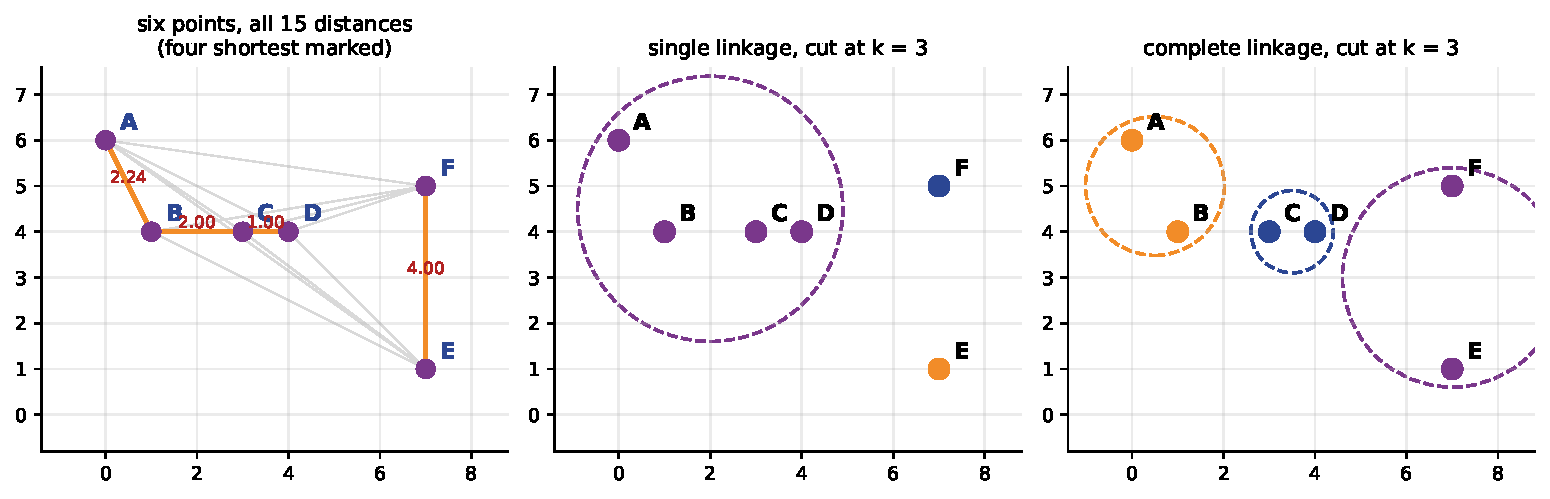
\includegraphics[width=\textwidth]{points.pdf}
  \caption{The six points that every hand calculation in these notes uses.
    Left: all fifteen pairwise distances, with the four shortest marked.
    Centre and right: the three-cluster partition each of the two linkages
    produces from exactly the same input. Single linkage strings $A$, $B$,
    $C$, $D$ into one cluster and leaves $E$ and $F$ alone; complete linkage
    finds three balanced pairs.}
  \label{fig:points}
\end{figure}

% =========================================================================
\section{A complete run by hand: single linkage}
\label{sec:single}

\subsection{The rule}

\textbf{Single linkage}, also called \textbf{nearest neighbour} or
\textbf{minimum} linkage, defines
\begin{equation}
  d_{\text{single}}(A, B) \;=\; \min_{a \in A,\ b \in B} d(a, b).
  \label{eq:single}
\end{equation}
Two clusters are as close as their closest pair of members. The consequence for
the algorithm is the update rule: when $A$ and $B$ merge, the distance from the
new cluster to any other cluster $K$ is
\begin{equation}
  d(A \cup B,\ K) \;=\; \min\bigl(d(A,K),\ d(B,K)\bigr).
  \label{eq:singleupd}
\end{equation}
Nothing is recomputed from the raw points: the new row of the matrix is the
element-wise minimum of the two old rows. This is the only arithmetic in the
whole run, and it is not really arithmetic.

\subsection{The run}

\begin{worked}[Single linkage on the six points, every step]
\textbf{Step 1.} The smallest entry in the full matrix is $d(C,D) = 1.0000$.
Merge them. The new row is the element-wise minimum of the $C$ and $D$ rows:
$\min(3.6056, 4.4721) = 3.6056$ against $A$, $\min(2, 3) = 2$ against $B$,
$\min(5.0000, 4.2426) = 4.2426$ against $E$, $\min(4.1231, 3.1623) = 3.1623$
against $F$.
\begin{center}\small
\begin{tabular}{lrrrrr}
  \toprule
  & $A$ & $B$ & $E$ & $F$ & $CD$ \\
  \midrule
  $A$  & --     & 2.2361 & 8.6023 & 7.0711 & 3.6056 \\
  $B$  & 2.2361 & --     & 6.7082 & 6.0828 & \textbf{2.0000} \\
  $E$  & 8.6023 & 6.7082 & --     & 4.0000 & 4.2426 \\
  $F$  & 7.0711 & 6.0828 & 4.0000 & --     & 3.1623 \\
  $CD$ & 3.6056 & \textbf{2.0000} & 4.2426 & 3.1623 & --  \\
  \bottomrule
\end{tabular}
\end{center}

\textbf{Step 2.} The smallest remaining entry is $d(B, CD) = 2.0000$ --- note
that this is smaller than $d(A,B) = 2.2361$, so $B$ joins the pair rather than
joining $A$. Merge.
\begin{center}\small
\begin{tabular}{lrrrr}
  \toprule
  & $A$ & $E$ & $F$ & $BCD$ \\
  \midrule
  $A$   & --     & 8.6023 & 7.0711 & \textbf{2.2361} \\
  $E$   & 8.6023 & --     & 4.0000 & 4.2426 \\
  $F$   & 7.0711 & 4.0000 & --     & 3.1623 \\
  $BCD$ & \textbf{2.2361} & 4.2426 & 3.1623 & -- \\
  \bottomrule
\end{tabular}
\end{center}

\textbf{Step 3.} Smallest is $d(A, BCD) = 2.2361$. Merge.
\begin{center}\small
\begin{tabular}{lrrr}
  \toprule
  & $E$ & $F$ & $ABCD$ \\
  \midrule
  $E$    & --     & 4.0000 & 4.2426 \\
  $F$    & 4.0000 & --     & \textbf{3.1623} \\
  $ABCD$ & 4.2426 & \textbf{3.1623} & -- \\
  \bottomrule
\end{tabular}
\end{center}

\textbf{Step 4.} Smallest is $d(F, ABCD) = 3.1623$ --- smaller than
$d(E,F) = 4.0000$, so $F$ abandons $E$ and joins the growing blob. Merge.
\begin{center}\small
\begin{tabular}{lrr}
  \toprule
  & $E$ & $ABCDF$ \\
  \midrule
  $E$     & --     & \textbf{4.0000} \\
  $ABCDF$ & \textbf{4.0000} & -- \\
  \bottomrule
\end{tabular}
\end{center}

\textbf{Step 5.} One entry left: $4.0000$. Merge. Done.

\medskip
\textbf{Merge heights, in order: $1.0000,\ 2.0000,\ 2.2361,\ 3.1623,\
4.0000$.} Every one of the five merges attached a \emph{single point} to the
one growing cluster. That is the shape single linkage likes, and it has a
name.
\end{worked}

\begin{keyidea}[Chaining]
Single linkage grows clusters by adding whichever point is nearest to
\emph{anything} already inside. Clusters therefore extend along paths of close
neighbours --- they \emph{chain}. On the six points the whole run is one chain.
Section~\ref{sec:shape} shows the same behaviour on 132 points, where it is
either exactly what you want or a complete disaster depending on the data.
\end{keyidea}

% =========================================================================
\section{The same six points, complete linkage}
\label{sec:complete}

\subsection{The rule}

\textbf{Complete linkage}, also called \textbf{farthest neighbour} or
\textbf{maximum} linkage, defines
\begin{equation}
  d_{\text{complete}}(A, B) \;=\; \max_{a \in A,\ b \in B} d(a, b),
  \label{eq:complete}
\end{equation}
with the update
\begin{equation}
  d(A \cup B,\ K) \;=\; \max\bigl(d(A,K),\ d(B,K)\bigr).
  \label{eq:completeupd}
\end{equation}
Two clusters are as far apart as their \emph{most distant} pair of members.
Merging two clusters is therefore only cheap if \emph{every} member of one is
close to \emph{every} member of the other, which is why complete linkage
produces compact, roughly equal-diameter clusters. The height at which a
cluster is formed is exactly its \textbf{diameter} --- the largest distance
between any two of its members.

\subsection{The run}

\begin{worked}[Complete linkage on the same six points]
\textbf{Step 1.} Identical to before: the smallest \emph{original} distance is
$d(C,D) = 1.0000$, and with all clusters singletons the linkage rule does not
matter yet. Merge. Now the new row is the element-wise \emph{maximum}:
$\max(3.6056, 4.4721) = 4.4721$ against $A$, $\max(2,3) = 3$ against $B$,
$\max(5.0000, 4.2426) = 5.0000$ against $E$, $\max(4.1231, 3.1623) = 4.1231$
against $F$.
\begin{center}\small
\begin{tabular}{lrrrrr}
  \toprule
  & $A$ & $B$ & $E$ & $F$ & $CD$ \\
  \midrule
  $A$  & --     & \textbf{2.2361} & 8.6023 & 7.0711 & 4.4721 \\
  $B$  & \textbf{2.2361} & --     & 6.7082 & 6.0828 & 3.0000 \\
  $E$  & 8.6023 & 6.7082 & --     & 4.0000 & 5.0000 \\
  $F$  & 7.0711 & 6.0828 & 4.0000 & --     & 4.1231 \\
  $CD$ & 4.4721 & 3.0000 & 5.0000 & 4.1231 & -- \\
  \bottomrule
\end{tabular}
\end{center}
Compare this with the step-1 matrix under single linkage. Four entries have
changed, and every one of them has \emph{grown}. Under single linkage
$d(B, CD)$ was $2.0000$; here it is $3.0000$, which is now larger than
$d(A,B) = 2.2361$. That single difference redirects the entire rest of the run.

\textbf{Step 2.} Smallest is $d(A,B) = 2.2361$. Merge --- and now $A$ and $B$
are a cluster, not $B$ and $CD$.
\begin{center}\small
\begin{tabular}{lrrrr}
  \toprule
  & $E$ & $F$ & $CD$ & $AB$ \\
  \midrule
  $E$  & --     & \textbf{4.0000} & 5.0000 & 8.6023 \\
  $F$  & \textbf{4.0000} & --     & 4.1231 & 7.0711 \\
  $CD$ & 5.0000 & 4.1231 & --     & 4.4721 \\
  $AB$ & 8.6023 & 7.0711 & 4.4721 & -- \\
  \bottomrule
\end{tabular}
\end{center}

\textbf{Step 3.} Smallest is $d(E,F) = 4.0000$. Merge.
\begin{center}\small
\begin{tabular}{lrrr}
  \toprule
  & $CD$ & $AB$ & $EF$ \\
  \midrule
  $CD$ & --     & \textbf{4.4721} & 5.0000 \\
  $AB$ & \textbf{4.4721} & --     & 8.6023 \\
  $EF$ & 5.0000 & 8.6023 & -- \\
  \bottomrule
\end{tabular}
\end{center}

\textbf{Step 4.} Smallest is $d(CD, AB) = 4.4721 = d(A,D)$, the largest of the
four cross distances $\{2.0000, 3.0000, 3.6056, 4.4721\}$. Merge.
\begin{center}\small
\begin{tabular}{lrr}
  \toprule
  & $EF$ & $ABCD$ \\
  \midrule
  $EF$   & --     & \textbf{8.6023} \\
  $ABCD$ & \textbf{8.6023} & -- \\
  \bottomrule
\end{tabular}
\end{center}

\textbf{Step 5.} Merge at $8.6023 = d(A,E)$, the largest distance in the whole
data. Done.

\medskip
\textbf{Merge heights, in order: $1.0000,\ 2.2361,\ 4.0000,\ 4.4721,\
8.6023$.} Three pairs form first, then the pairs combine. No chain anywhere.
\end{worked}

\subsection{Compare the two}

\begin{center}\small
\begin{tabular}{clrlr}
  \toprule
  step & single-linkage merge & height & complete-linkage merge & height \\
  \midrule
  1 & $\{C\} + \{D\}$    & 1.0000 & $\{C\} + \{D\}$      & 1.0000 \\
  2 & $\{B\} + \{CD\}$   & 2.0000 & $\{A\} + \{B\}$      & 2.2361 \\
  3 & $\{A\} + \{BCD\}$  & 2.2361 & $\{E\} + \{F\}$      & 4.0000 \\
  4 & $\{F\} + \{ABCD\}$ & 3.1623 & $\{CD\} + \{AB\}$    & 4.4721 \\
  5 & $\{E\} + \{FABCD\}$& 4.0000 & $\{EF\} + \{CDAB\}$  & 8.6023 \\
  \bottomrule
\end{tabular}
\end{center}

Two things to notice. First, the trees agree only at step 1 and then diverge
completely. Second, \textbf{complete-linkage heights are always at least as
large as single-linkage heights} at the same stage --- a maximum over the same
set of cross distances cannot be below the minimum --- so a complete-linkage
dendrogram is stretched vertically. Never compare a height from one linkage
with a height from another; they are not in the same units of meaning.

The flat clusterings tell the story most sharply:

\begin{lstlisting}
def groups(lab):                    # label vector -> readable set notation
    return " ".join("{" + "".join(LBL[i] for i in range(6) if lab[i] == g)
                    + "}" for g in sorted(set(lab)))

for k in (2, 3, 4):
    print("k = %d   single  : %s" % (k, groups(fcluster(Zs, k, "maxclust"))))
    print("        complete: %s" % groups(fcluster(Zc, k, "maxclust")))
\end{lstlisting}
\begin{codeout}
k = 2   single  : {ABCDF} {E}
        complete: {EF} {ABCD}
k = 3   single  : {ABCD} {F} {E}
        complete: {EF} {CD} {AB}
k = 4   single  : {BCD} {A} {F} {E}
        complete: {E} {F} {CD} {AB}
\end{codeout}

At $k = 2$ single linkage produces a cluster of five and a singleton; complete
linkage produces four and two. At $k = 3$ single linkage produces one cluster
and two singletons; complete linkage produces three balanced pairs. Same six
points, same Euclidean distances, opposite personalities.

\begin{figure}[htbp]
  \centering
  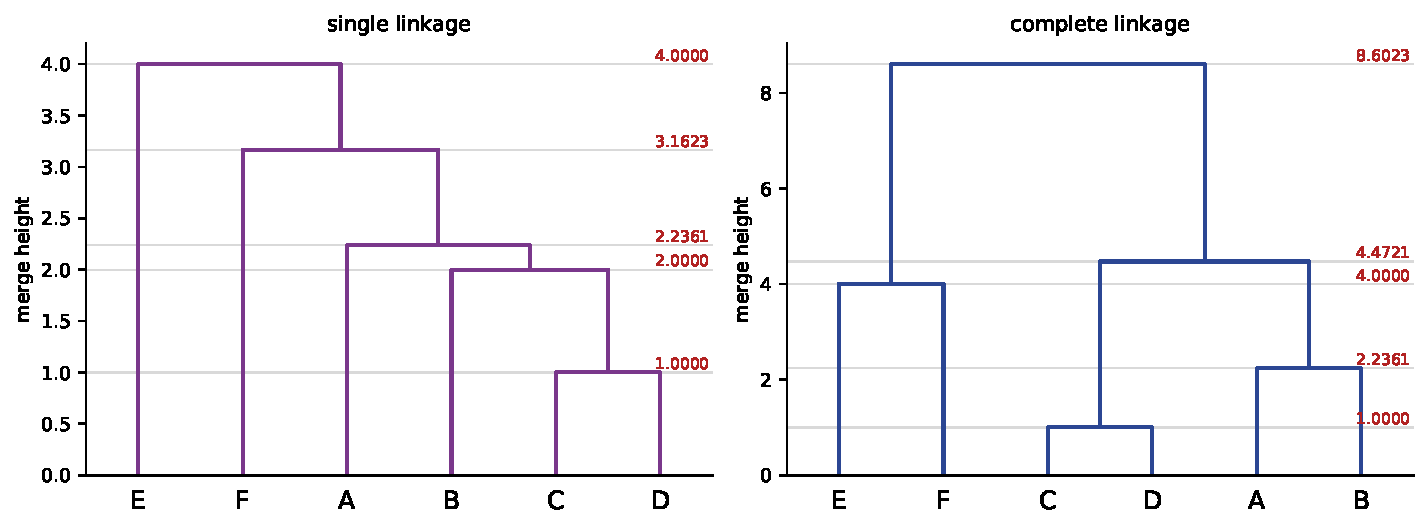
\includegraphics[width=\textwidth]{dendro6.pdf}
  \caption{The two dendrograms, drawn from the merge heights computed above.
    Left, single linkage: a staircase, each step adding one point --- the
    signature of chaining. Right, complete linkage: three pairs, then two
    groups, then the root at $8.6023 = d(A,E)$, the diameter of the whole set.
    Note that the vertical scales differ by a factor of two.}
  \label{fig:dendro6}
\end{figure}

\begin{caution}[Ties]
These six points were chosen so that all fifteen distances differ. Real data
--- especially data on an integer grid, or with duplicated rows --- has ties,
and then the merge order is \textbf{implementation-dependent}. Two correct
programs can return two different trees. SciPy's documentation says so
explicitly. If an examination question has a tie, say which choice you made
and carry on; if a laboratory result changes when you change library version,
check for ties before assuming you have a bug.
\end{caution}

% =========================================================================
\section{The library agrees}
\label{sec:scipy}

\subsection{The linkage matrix}

\texttt{scipy.cluster.hierarchy.linkage} returns an $(n-1) \times 4$ array
$Z$. Row $t$ says: cluster \texttt{Z[t,0]} and cluster \texttt{Z[t,1]} merged
at height \texttt{Z[t,2]}, and the result contains \texttt{Z[t,3]} original
observations. Cluster indices below $n$ are the original points; index $n+t$
is the cluster created at row $t$. That indexing convention is the only
awkward part of the API and it is worth ten seconds of attention now.

\begin{lstlisting}
Zs, Zc = linkage(P6, method="single"), linkage(P6, method="complete")
print("step  single-linkage merge            height   "
      "complete-linkage merge          height")
ns, nc = list(LBL), list(LBL)          # decode the index convention
for t in range(5):
    a, b, h, _ = Zs[t]
    a2, b2, h2, _ = Zc[t]
    m1 = "{%s} + {%s}" % (ns[int(a)], ns[int(b)])
    m2 = "{%s} + {%s}" % (nc[int(a2)], nc[int(b2)])
    print("  %d   %-30s %7.4f   %-30s %7.4f" % (t + 1, m1, h, m2, h2))
    ns.append(ns[int(a)] + ns[int(b)])
    nc.append(nc[int(a2)] + nc[int(b2)])
\end{lstlisting}
\begin{codeout}
step  single-linkage merge            height   complete-linkage merge          height
  1   {C} + {D}                       1.0000   {C} + {D}                       1.0000
  2   {B} + {CD}                      2.0000   {A} + {B}                       2.2361
  3   {A} + {BCD}                     2.2361   {E} + {F}                       4.0000
  4   {F} + {ABCD}                    3.1623   {CD} + {AB}                     4.4721
  5   {E} + {FABCD}                   4.0000   {EF} + {CDAB}                   8.6023
\end{codeout}

\begin{tryit}[Check the hand run against the library]
The script that produced these notes implements the loop of
Section~\ref{sec:hac} in plain Python --- rescan the matrix, find the minimum,
take the element-wise min or max, repeat --- and compares the heights it gets
with SciPy's:
\begin{lstlisting}
merge heights in order: 1.0000, 2.0000, 2.2361, 3.1623, 4.0000
scipy heights          : 1.0000, 2.0000, 2.2361, 3.1623, 4.0000
match to 1e-12: True
\end{lstlisting}
and the same for complete linkage:
\begin{lstlisting}
merge heights in order: 1.0000, 2.2361, 4.0000, 4.4721, 8.6023
scipy heights          : 1.0000, 2.2361, 4.0000, 4.4721, 8.6023
match to 1e-12: True
\end{lstlisting}
Write the loop yourself. It is about twenty lines and it is the fastest way to
be certain you have understood the algorithm.
\end{tryit}

\subsection{Three routes to the same flat clustering}

\begin{lstlisting}
X, y = load_iris(return_X_y=True)
Xs = StandardScaler().fit_transform(X)
Z = linkage(Xs, method="ward")
a = fcluster(Z, 3, "maxclust")                 # scipy, from the tree
b = cut_tree(Z, n_clusters=3).ravel()          # scipy, same tree
c = AgglomerativeClustering(n_clusters=3, linkage="ward").fit_predict(Xs)
\end{lstlisting}
\begin{codeout}
  scipy fcluster        sizes 49,30,71
  scipy cut_tree        sizes 49,30,71
  sklearn Agglomerative sizes 71,49,30
  fcluster vs cut_tree  ARI 1.0000
  fcluster vs sklearn   ARI 1.0000
\end{codeout}

The three agree exactly; only the arbitrary cluster \emph{numbering} differs,
which is why the sizes are permuted and the adjusted Rand index --- a measure
of agreement between partitions that ignores labels --- is $1.0000$. Use
\texttt{scipy} when you want the tree and the dendrogram; use
\texttt{AgglomerativeClustering} when you want a step in a
\texttt{Pipeline}. Do not expect \texttt{AgglomerativeClustering} to give you
the tree: it computes only as much of it as \texttt{n\_clusters} requires,
unless you pass \texttt{distance\_threshold=0} and
\texttt{n\_clusters=None}.

% =========================================================================
\section{The distance between two clusters}
\label{sec:linkage}

This is the definitional heart of the lecture. Everything else is consequence.

Let $A$ and $B$ be clusters with $n_A$ and $n_B$ members and centroids
$c_A = \frac{1}{n_A}\sum_{a \in A} a$ and $c_B$. The five standard rules are:

\begin{align}
  d_{\text{single}}(A,B)   &= \min_{a \in A, b \in B} d(a,b)
    &&\text{nearest neighbour} \label{eq:l1}\\
  d_{\text{complete}}(A,B) &= \max_{a \in A, b \in B} d(a,b)
    &&\text{farthest neighbour} \label{eq:l2}\\
  d_{\text{average}}(A,B)  &= \frac{1}{n_A n_B}\sum_{a \in A}\sum_{b \in B} d(a,b)
    &&\text{UPGMA} \label{eq:l3}\\
  d_{\text{centroid}}(A,B) &= \lVert c_A - c_B \rVert_2
    &&\text{UPGMC} \label{eq:l4}\\
  d_{\text{ward}}(A,B)     &= \sqrt{\frac{2\,n_A n_B}{n_A + n_B}}\;
                              \lVert c_A - c_B \rVert_2
    &&\text{minimum variance} \label{eq:l5}
\end{align}

The first three are defined for \emph{any} dissimilarity: they only ever look
up entries of $D$. The last two need the points themselves, in a space where
averaging makes sense --- they are Euclidean-only.

\begin{figure}[htbp]
  \centering
  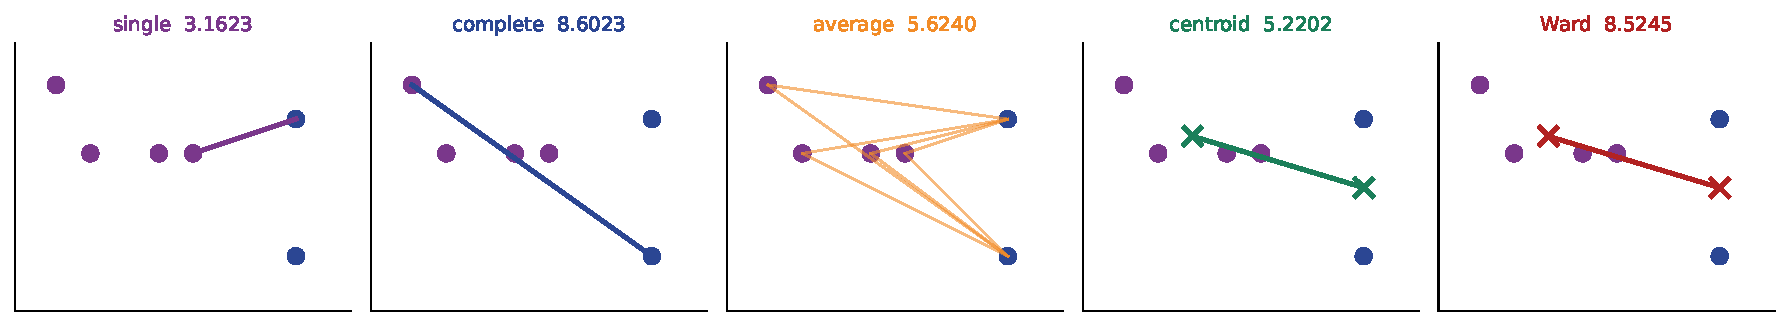
\includegraphics[width=\textwidth]{whatmeasured.pdf}
  \caption{The five rules, all measuring the distance between the same two
    clusters $A = \{A,B,C,D\}$ (purple) and $B = \{E,F\}$ (blue) on the six
    points. Single takes one cross distance, complete takes another, average
    takes all eight, and centroid and Ward work from the two centroids
    (crosses).}
  \label{fig:whatmeasured}
\end{figure}

\begin{worked}[All five, for $A = \{A,B,C,D\}$ against $B = \{E,F\}$]
There are $4 \times 2 = 8$ cross distances. From the initial matrix:
\[
  \{8.6023,\ 7.0711,\ 6.7082,\ 6.0828,\ 5.0000,\ 4.1231,\ 4.2426,\ 3.1623\}
\]
in the order $AE, AF, BE, BF, CE, CF, DE, DF$. Therefore
\begin{itemize}[leftmargin=*]
  \item \textbf{single} $= \min = 3.1623$ \quad (the pair $D,F$)
  \item \textbf{complete} $= \max = 8.6023$ \quad (the pair $A,E$)
  \item \textbf{average} $= \dfrac{44.9924}{8} = 5.6240$
  \item \textbf{centroid}: $c_A = \frac{1}{4}(0+1+3+4,\ 6+4+4+4) = (2.0,\
    4.5)$ and $c_B = \frac{1}{2}(7+7,\ 1+5) = (7.0,\ 3.0)$, so
    $\lVert c_A - c_B\rVert = \sqrt{5^2 + 1.5^2} = \sqrt{27.25} = 5.2202$
  \item \textbf{Ward}: $\dfrac{2 \cdot 4 \cdot 2}{4+2} = \dfrac{16}{6} =
    2.6667$, so $d = \sqrt{2.6667} \times 5.2202 = 1.6330 \times 5.2202 =
    8.5245$
\end{itemize}
Five numbers between $3.16$ and $8.60$, all describing the same pair of
clusters. The library confirms every one:
\begin{lstlisting}
  single   min          = 3.1623
  complete max          = 8.6023
  average  mean         = 5.6240
  centroid ||cA - cB||  = 5.2202   cA = (2.0000, 4.5000)  cB = (7.0000, 3.0000)
  ward     sqrt(2*nA*nB/(nA+nB))*||cA-cB|| = sqrt(2.6667)*5.2202 = 8.5245
\end{lstlisting}
\end{worked}

\subsection{Where Ward's formula comes from}

Ward's method is the only one of the five that is derived from an
\emph{objective}. Define the within-cluster sum of squares (the ``error sum of
squares'', ESS) of a cluster as
\begin{equation}
  \mathrm{ESS}(A) = \sum_{a \in A} \lVert a - c_A \rVert^2 ,
  \label{eq:ess}
\end{equation}
and the total for a partition as the sum over its clusters. At the singleton
level the total is $0$; at the root it is the total variance of the data times
$n$. Every merge increases it. Ward's rule is: \textbf{merge the pair that
increases the total ESS by the least.} The increase has a closed form:
\begin{equation}
  \Delta(A,B) \;=\; \mathrm{ESS}(A \cup B) - \mathrm{ESS}(A) - \mathrm{ESS}(B)
  \;=\; \frac{n_A n_B}{n_A + n_B}\,\lVert c_A - c_B \rVert^2 .
  \label{eq:wardcost}
\end{equation}
SciPy reports $\sqrt{2\Delta}$ as the merge height, which is what
equation~\eqref{eq:l5} says; the factor is chosen so that for two singletons
the height is just $d(a,b)$, since then $\Delta = \tfrac12 d^2$. Check it on
the worked example: $\Delta = \frac{4 \cdot 2}{6}\times 27.25 = 36.3333$, and
$\sqrt{2 \times 36.3333} = 8.5245$. Which is what the library printed.

\begin{keyidea}
Ward is $k$-means' objective run greedily bottom-up. It merges whichever pair
costs the least extra within-cluster variance. That is why it produces
compact, similarly sized, roughly spherical clusters, and why it is almost
always the sensible default on numeric data.
\end{keyidea}

\begin{caution}[Ward and centroid need Euclidean distances]
Equations~\eqref{eq:l4} and~\eqref{eq:l5} contain a centroid, and a centroid
only means something in a vector space. SciPy will \emph{not stop you} from
passing a precomputed city-block or cosine matrix to
\texttt{method="ward"}. It runs, it returns a tree, and the numbers have no
variance interpretation whatever. On the wine data it even scored well
(Section~\ref{sec:cut}) --- which is exactly why the mistake survives. Use
average or complete linkage for a non-Euclidean dissimilarity.
\end{caution}

% =========================================================================
\section{One formula for all five: Lance--Williams}
\label{sec:lw}

Recomputing $d(A \cup B, K)$ from the raw points after every merge would be
expensive and, for a precomputed matrix, impossible. Lance and Williams showed
in 1967 that for all the standard linkages the new distance can be written in
terms of the \emph{three numbers already in the matrix}:
\begin{equation}
  d(A \cup B,\ K) \;=\; \alpha_A\, d(A,K) \;+\; \alpha_B\, d(B,K)
  \;+\; \beta\, d(A,B) \;+\; \gamma\, \bigl| d(A,K) - d(B,K) \bigr| .
  \label{eq:lw}
\end{equation}
With $n_A$, $n_B$, $n_K$ the cluster sizes and $T = n_A + n_B + n_K$:

\begin{center}
\begin{tabular}{lllll}
  \toprule
  method & $\alpha_A$ & $\alpha_B$ & $\beta$ & $\gamma$ \\
  \midrule
  single   & $1/2$ & $1/2$ & $0$ & $-1/2$ \\
  complete & $1/2$ & $1/2$ & $0$ & $+1/2$ \\
  average  & $n_A/(n_A{+}n_B)$ & $n_B/(n_A{+}n_B)$ & $0$ & $0$ \\
  centroid & $n_A/(n_A{+}n_B)$ & $n_B/(n_A{+}n_B)$ &
             $-n_A n_B/(n_A{+}n_B)^2$ & $0$ \\
  Ward     & $(n_A{+}n_K)/T$ & $(n_B{+}n_K)/T$ & $-n_K/T$ & $0$ \\
  \bottomrule
\end{tabular}
\end{center}

\textbf{Centroid and Ward operate on squared distances}: feed the recurrence
$d^2$ and take a square root at the end. The other three operate on the
distances directly.

\begin{worked}[Single and complete drop out of the formula]
Put $\alpha_A = \alpha_B = 1/2$, $\beta = 0$, $\gamma = -1/2$ into
\eqref{eq:lw} and write $u = d(A,K)$, $v = d(B,K)$:
\[
  \tfrac12 u + \tfrac12 v - \tfrac12|u-v| = \tfrac{u+v-|u-v|}{2} = \min(u,v),
\]
because if $u \le v$ then $|u-v| = v-u$ and the expression is
$(u+v-v+u)/2 = u$. Flip the sign of $\gamma$ and the same algebra gives
$\max(u,v)$. So equations~\eqref{eq:singleupd} and~\eqref{eq:completeupd} are
special cases of one recurrence. \ensuremath{\square}
\end{worked}

\begin{tryit}[Reimplement all five from the recurrence alone]
Write a loop that never touches the coordinates after the first
\texttt{pdist} --- only \eqref{eq:lw} --- and check it against SciPy:
\begin{lstlisting}
for method in ("single", "complete", "average", "centroid", "ward"):
    h = lance_williams(P6, method)
    print(method, h, linkage(P6, method=method)[:, 2])
\end{lstlisting}
\begin{codeout}
  single    LW 1.0000 2.0000 2.2361 3.1623 4.0000 | scipy 1.0000 2.0000 2.2361 3.1623 4.0000 | match True
  complete  LW 1.0000 2.2361 4.0000 4.4721 8.6023 | scipy 1.0000 2.2361 4.0000 4.4721 8.6023 | match True
  average   LW 1.0000 2.2361 3.2694 4.0000 5.6240 | scipy 1.0000 2.2361 3.2694 4.0000 5.6240 | match True
  centroid  LW 1.0000 2.2361 3.1623 4.0000 5.2202 | scipy 1.0000 2.2361 3.1623 4.0000 5.2202 | match True
  ward      LW 1.0000 2.2361 4.0000 4.4721 8.5245 | scipy 1.0000 2.2361 4.0000 4.4721 8.5245 | match True
\end{codeout}
Notice the last average-linkage height, $5.6240$: that is the mean of the
eight cross distances computed by hand in Section~\ref{sec:linkage}, arrived
at by the recurrence without ever revisiting a raw point.
\end{tryit}

\begin{keyidea}
Lance--Williams is why one $O(n^2)$-memory implementation serves every
linkage: the merge loop is identical and only four constants change. It is
also why the proximity matrix is the only thing HAC ever needs to keep.
\end{keyidea}

Here is what the five do on our six points, side by side:

\begin{codeout}
  single    C+D@1.000  B+CD@2.000  A+BCD@2.236  F+ABCD@3.162  E+FABCD@4.000
  complete  C+D@1.000  A+B@2.236  E+F@4.000  CD+AB@4.472  EF+CDAB@8.602
  average   C+D@1.000  A+B@2.236  CD+AB@3.269  E+F@4.000  CDAB+EF@5.624
  centroid  C+D@1.000  A+B@2.236  CD+AB@3.162  E+F@4.000  CDAB+EF@5.220
  ward      C+D@1.000  A+B@2.236  E+F@4.000  CD+AB@4.472  EF+CDAB@8.524
\end{codeout}

Average, centroid and Ward all recover the sensible answer $\{A,B,C,D\}$ and
$\{E,F\}$ at $k=2$; only single linkage does not. The three heights they
report for the final merge --- $5.624$, $5.220$, $8.524$ --- are the mean
cross distance, the centroid distance, and $\sqrt{2\Delta}$, exactly as
computed by hand above.

% =========================================================================
\section{What each linkage does to cluster shape}
\label{sec:shape}

\subsection{Three shapes, five linkages}

Figure~\ref{fig:linkgrid} runs all five on three synthetic problems where the
right answer is known, so the adjusted Rand index (ARI) --- $1$ for a perfect
match with the truth, $0$ for chance --- can be measured. Read it as a
character sketch of each method.

\begin{figure}[htbp]
  \centering
  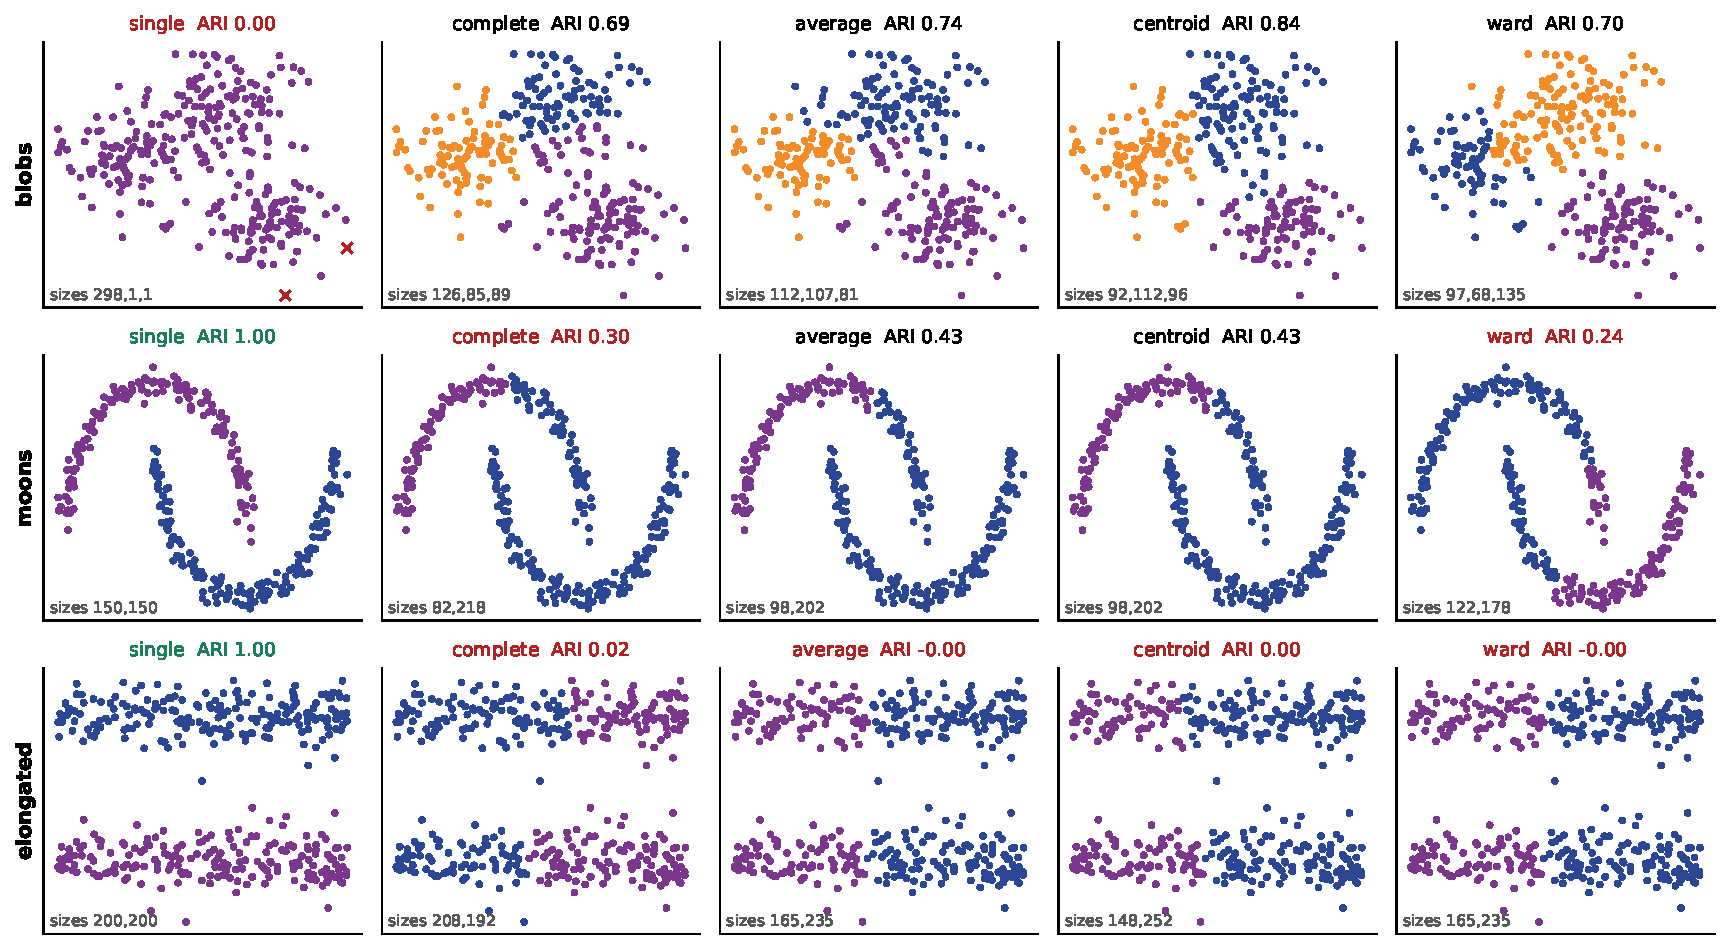
\includegraphics[width=\textwidth]{linkgrid.pdf}
  \caption{Five linkages on three problems. Red crosses mark clusters of three
    points or fewer. Top row, three Gaussian blobs: single linkage returns
    $298$/$1$/$1$ and an ARI of $0.000$. Middle row, two interleaved moons:
    only single linkage gets it, at ARI $1.000$. Bottom row, two long thin
    bands: same story, and every compact linkage cuts them the wrong way
    across the middle.}
  \label{fig:linkgrid}
\end{figure}

\begin{codeout}
data        linkage      ARI    sizes
blobs       single     0.000  298,1,1
blobs       complete   0.692 126,85,89
blobs       average    0.741 112,107,81
blobs       centroid   0.844  92,112,96
blobs       ward       0.697  97,68,135

moons       single     1.000  150,150
moons       complete   0.297   82,218
moons       average    0.425   98,202
moons       centroid   0.425   98,202
moons       ward       0.241  122,178

elongated   single     1.000  200,200
elongated   complete   0.017  208,192
elongated   average   -0.002  165,235
elongated   centroid   0.004  148,252
elongated   ward      -0.002  165,235
\end{codeout}

Three lessons, in increasing order of importance.

\textbf{Single linkage is the only one that can follow a non-convex shape.}
On the moons and on the two long bands it is perfect and everything else is
near-random. It gets there by chaining: it walks along the arc one nearest
neighbour at a time, and the arc's shape is irrelevant. No linkage based on
centroids or diameters can do that, because both moons have almost the same
centroid.

\textbf{Single linkage falls apart the moment the clusters overlap or there
are outliers.} On three Gaussian blobs it returns one cluster of $298$ and two
singletons and an ARI of $0.000$. The blobs touch, so the chain runs straight
from one into the next; the only merges left for the top of the tree are the
two most isolated points. This is not a bug and it is not a bad random seed:
it is what nearest-neighbour linkage does whenever the between-cluster gap is
not larger than the within-cluster spacing.

\textbf{Complete linkage and Ward break elongated clusters.} Look at the
bottom row. The truth is two horizontal bands; complete linkage and Ward
return a left half and a right half. They are not confused --- they are doing
their job. A method that minimises diameter, or minimises within-cluster
variance, genuinely prefers two compact halves to two long thin bands, because
the bands have enormous diameter and variance. The mismatch is between the
objective and the data, not inside the algorithm.

\begin{keyidea}
The linkage rule is not a tuning knob. It is a statement about what shape you
believe a cluster has. Single linkage says ``connected''. Complete linkage
says ``small diameter''. Ward says ``low variance''. Choose the one whose
belief matches your problem, and expect nonsense if you choose wrongly.
\end{keyidea}

\subsection{The chaining failure, measured}

The moons result makes chaining look like a superpower. Here is the price.

Take two well-separated Gaussian clusters of sixty points, at $x = 0$ and
$x = 8$, each with standard deviation $0.45$. The closest point of one to the
closest point of the other is $5.5714$ apart. Every linkage separates them
perfectly. Now scatter a handful of noise points in a line between them and
watch what happens.

\begin{lstlisting}
def bridge_data(nb, n=60, seed=3):   # seed=3 fixes the dataset, not a run
    rng = np.random.default_rng(seed)
    left  = np.c_[rng.normal(0, 0.45, n), rng.normal(0, 0.45, n)]
    right = np.c_[rng.normal(8, 0.45, n), rng.normal(0, 0.45, n)]
    X, mark = np.vstack([left, right]), np.r_[np.zeros(n), np.ones(n)]
    if nb:                           # nb noise points strung along the gap
        X = np.vstack([X, np.c_[np.linspace(1, 7, nb),
                                rng.normal(0, 0.06, nb)]])
        mark = np.r_[mark, np.full(nb, 2)]
    return X, mark.astype(int)

print("bridge  linkage    height at which the two true clusters fuse   "
      "k = 2 sizes   ARI")
for nb in (0, 4, 8, 12, 16):
    X, mark = bridge_data(nb)        # 120 real points + nb bridge points
    for m in ("single", "complete", "ward"):
        Z = linkage(X, method=m)
        lab = fcluster(Z, 2, "maxclust")
        sz = sorted(np.bincount(lab)[1:].tolist(), reverse=True)
        print("%4d    %-9s %36.3f   %-12s %.3f"
              % (nb, m, fuse_height(Z, len(X), mark), str(sz),
                 adjusted_rand_score(mark[:120], lab[:120])))
    print()
\end{lstlisting}
\begin{codeout}
bridge  linkage    height at which the two true clusters fuse   k = 2 sizes   ARI
   0    single                                   5.571   [60, 60]     1.000
   0    complete                                10.381   [60, 60]     1.000
   0    ward                                    62.573   [60, 60]     1.000

   4    single                                   2.005   [62, 62]     1.000
   4    complete                                10.381   [63, 61]     1.000
   4    ward                                    62.334   [63, 61]     1.000

   8    single                                   0.869   [67, 61]     1.000
   8    complete                                10.381   [64, 64]     1.000
   8    ward                                    61.918   [66, 62]     1.000

  12    single                                   0.565   [131, 1]     0.000
  12    complete                                10.381   [70, 62]     1.000
  12    ward                                    61.146   [70, 62]     1.000

  16    single                                   0.434   [135, 1]     0.000
  16    complete                                10.381   [70, 66]     1.000
  16    ward                                    61.183   [72, 64]     1.000
\end{codeout}

Read the single-linkage column downwards: $5.571 \to 2.005 \to 0.869 \to
0.565 \to 0.434$. Twelve points --- ten per cent of the data, none of them
anywhere near either cluster --- pull the fusion height down by a factor of
ten, and at that point the two-cluster answer stops being $[60,60]$ and
becomes $[131, 1]$: everything in one cluster, plus one stray point. The ARI
falls from $1.000$ to $0.000$.

The complete and Ward columns do not move at all. Complete linkage fuses at
$10.381$ whatever you do, because that number is $\max_{a,b} d(a,b)$ across
the two clusters and no bridge point can reduce a maximum.

Why does single linkage collapse? Because it never has to pay the $5.5714$
gap. It walks:

\begin{codeout}
  nb  spacing  bottleneck step on the left-bridge-right path  single fuse height
   0      nan                          5.5714               5.5714
   4   2.0000                          2.0021               2.0048
   8   0.8571                          0.8687               0.8687
  12   0.5455                          0.5634               0.5653
  16   0.4000                          0.4242               0.4341
\end{codeout}

The fuse height is exactly the largest single step along the chain
left$\to$bridge$\to$right --- the bottleneck of the path. Bridge spacing
$0.5455$ gives fuse height $0.5653$. Single linkage is measuring
\emph{connectivity}, and a thin bridge is a connection.

\begin{figure}[htbp]
  \centering
  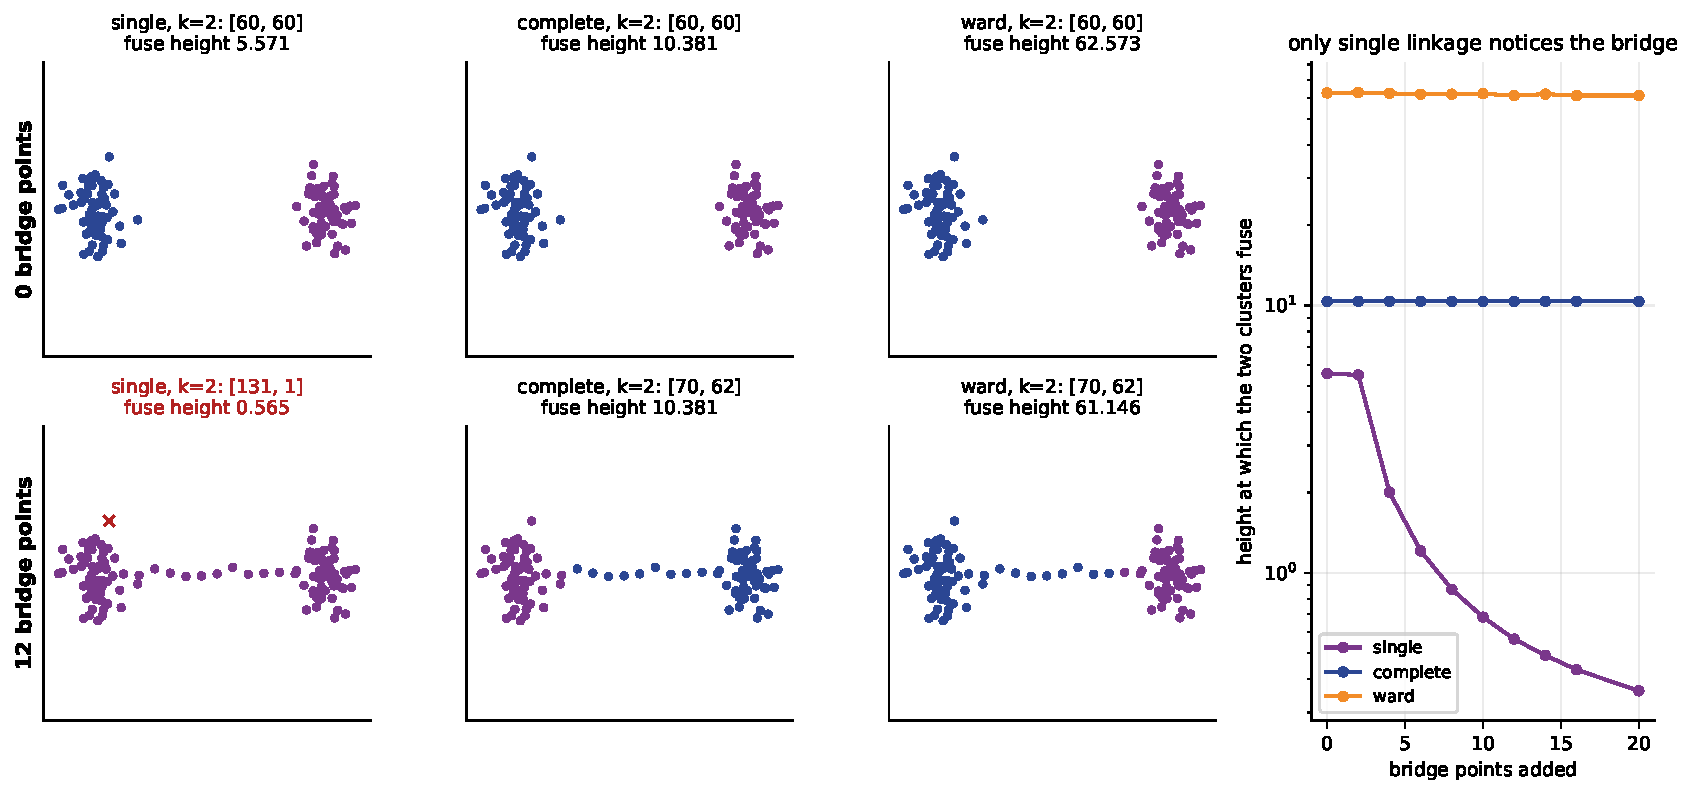
\includegraphics[width=\textwidth]{chaining.pdf}
  \caption{Chaining. Top row: two clean clusters; all three linkages give
    $[60, 60]$. Bottom row: twelve bridge points added. Single linkage now
    returns $[131, 1]$ --- one giant cluster and the red cross --- while
    complete and Ward are unmoved. Right: the fusion height as bridge points
    are added, on a log scale. Only the purple line moves.}
  \label{fig:chaining}
\end{figure}

\begin{caution}[This is the single most examinable weakness of HAC]
``Single linkage suffers from the chaining effect'' is a sentence you can
write without understanding it. The version that earns marks names the
mechanism: the linkage takes a \emph{minimum} over cross pairs, so a
\emph{single} short link is enough to fuse two clusters, and a path of noise
points supplies one. Complete and average linkage cannot be fooled this way
because a maximum, or a mean over $n_A n_B$ pairs, cannot be dragged down by
one pair.
\end{caution}

% =========================================================================
\section{Centroid linkage can go backwards}
\label{sec:inv}

Every dendrogram you have seen so far has heights that increase from the
leaves to the root. That property is called \textbf{monotonicity}, and it is
what makes the picture readable: cutting at a height gives a well-defined set
of clusters, and ``merged early'' means ``merged at a small distance''.

Single, complete, average and Ward linkage are all guaranteed monotone. They
are \textbf{reducible}: if $A$ and $B$ are each at least $\delta$ from $K$,
then $A \cup B$ is at least $\delta$ from $K$ too, so a merge can never create
a shorter distance than the one just used. Centroid linkage is not reducible,
and the counterexample fits on three points.

\begin{worked}[An inversion on three points]
Take $P_1 = (0,0)$, $P_2 = (1,0)$, $P_3 = (0.48, 0.84)$ --- almost, but not
quite, an equilateral triangle. The three distances are
\[
  d(P_1,P_2) = 1.0000, \qquad d(P_1,P_3) = 0.9675, \qquad d(P_2,P_3) = 0.9879 .
\]
The smallest is $d(P_1,P_3) = 0.9675$, so merge $P_1$ and $P_3$ at height
$0.9675$. Their centroid is
\[
  c = \tfrac12\bigl((0,0) + (0.48, 0.84)\bigr) = (0.2400,\ 0.4200),
\]
and the distance from that centroid to the remaining point $P_2 = (1,0)$ is
\[
  \sqrt{(1 - 0.24)^2 + (0 - 0.42)^2} = \sqrt{0.5776 + 0.1764}
  = \sqrt{0.7540} = 0.8683 .
\]
So the second and final merge happens at height $\mathbf{0.8683}$ ---
\textbf{lower than the first merge at $0.9675$}. The dendrogram goes
\emph{down}. The drop is $0.0991$.
\end{worked}

\begin{codeout}
scipy centroid heights: 0.9675 0.8683
monotone: False   drop = 0.0991
  single    0.9675 0.9879  monotone True
  complete  0.9675 1.0000  monotone True
  average   0.9675 0.9940  monotone True
  ward      0.9675 1.0027  monotone True
\end{codeout}

The geometry is simple once seen: the centroid of two merged points sits
\emph{between} them, and so is closer to everything else than at least one of
them was. Averaging moves you inward. Ward avoids the problem because its
$\sqrt{2 n_A n_B/(n_A+n_B)}$ factor grows with cluster size and more than
compensates for the inward move.

\begin{figure}[htbp]
  \centering
  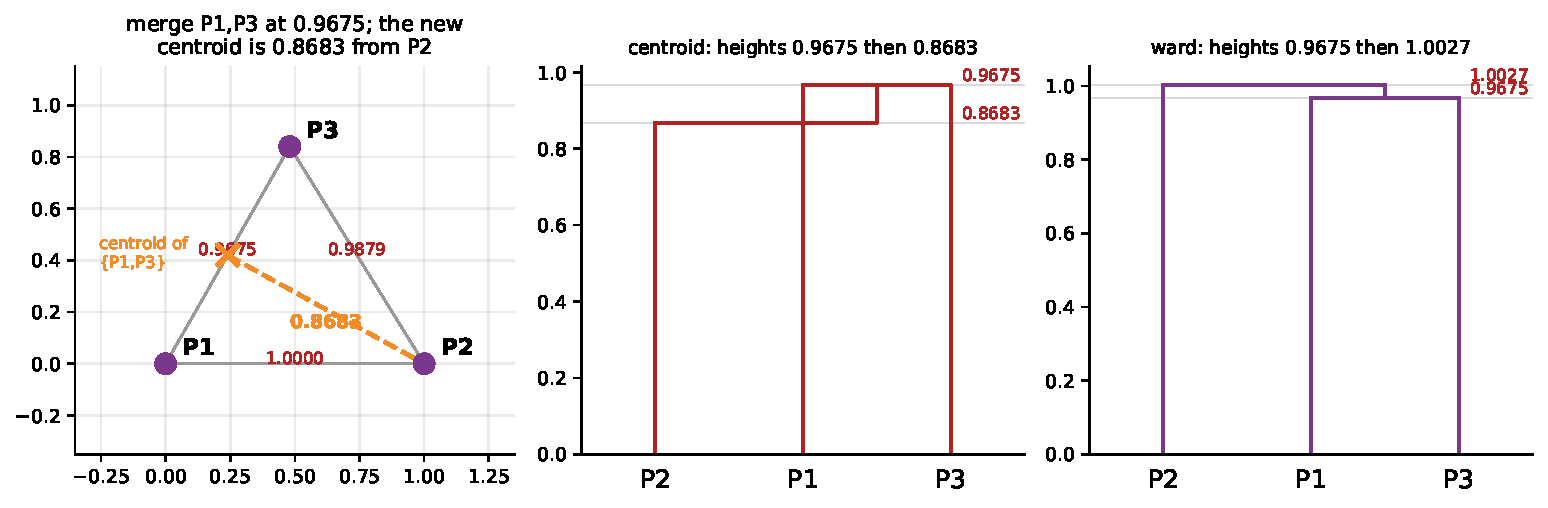
\includegraphics[width=\textwidth]{inversion.pdf}
  \caption{Left: the three points, with the merged pair's centroid marked by a
    cross; the dashed orange line ($0.8683$) is shorter than either original
    side of the triangle involving $P_2$. Centre: the centroid dendrogram,
    which descends. Right: Ward on the same three points, which does not.}
  \label{fig:inversion}
\end{figure}

This is not a pathological corner case. On uniformly random points it is the
normal state of affairs. Note the shape of this experiment: \emph{every trial
draws a new point set} --- the variation across trials is the measurement ---
but all $1600$ draws come off one stream with one seed, so the percentages
below are exactly what you will get:

\begin{lstlisting}
rng = np.random.default_rng(0)       # one seed; each trial draws a new set
for n in (5, 10, 25, 50):
    bad = 0
    for _ in range(400):
        h = linkage(rng.uniform(0, 1, size=(n, 2)), method="centroid")[:, 2]
        bad += int(np.any(np.diff(h) < -1e-12))
    print(n, bad, 100 * bad / 400)
\end{lstlisting}
\begin{codeout}
  n =  5 uniform points:  25 of 400 trees have an inversion (6.2%)
  n = 10 uniform points:  89 of 400 trees have an inversion (22.2%)
  n = 25 uniform points: 218 of 400 trees have an inversion (54.5%)
  n = 50 uniform points: 302 of 400 trees have an inversion (75.5%)
\end{codeout}

\begin{figure}[htbp]
  \centering
  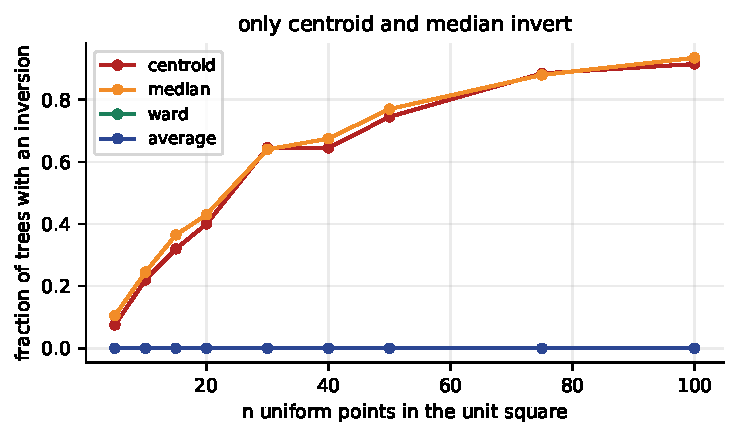
\includegraphics[width=0.62\textwidth]{inversionrate.pdf}
  \caption{Fraction of trees containing at least one inversion, over $200$
    random point sets per value of $n$. Centroid and median linkage invert
    routinely; average and Ward never do.}
  \label{fig:inversionrate}
\end{figure}

\begin{caution}[What an inversion costs you]
A non-monotone dendrogram cannot be read the usual way. ``Cut at height $h$''
is no longer well defined, because a cluster formed at $0.97$ may sit
\emph{underneath} an edge drawn at $0.87$, and the connected components below
a horizontal line stop matching the merge sequence. Use centroid linkage only
if you have a specific reason to; average linkage answers almost the same
question and is monotone.
\end{caution}

% =========================================================================
\section{Cutting the dendrogram}
\label{sec:cut}

\subsection{Two ways to cut}

A tree is not a clustering. To get one, cut it.

\textbf{By count.} \texttt{fcluster(Z, k, criterion="maxclust")} returns the
partition with (at most) $k$ clusters --- equivalently, stop the algorithm
after $n-k$ merges.

\textbf{By height.} \texttt{fcluster(Z, t, criterion="distance")} cuts the
tree at height $t$ and returns the connected components below. You get however
many clusters that produces.

They are the same operation seen from two sides, and on iris with Ward linkage
they line up like this:

\begin{codeout}
  cut at height   4.0 -> 8 clusters, sizes 20,7,22,5,25,45,8,18
  cut at height   6.0 -> 5 clusters, sizes 20,29,30,45,26
  cut at height   8.0 -> 4 clusters, sizes 49,30,45,26
  cut at height  10.0 -> 3 clusters, sizes 49,30,71
  cut at height  12.0 -> 3 clusters, sizes 49,30,71
  cut at height  16.0 -> 2 clusters, sizes 49,101
\end{codeout}

Cutting at $10$ and at $12$ give the same answer, because no merge happens
between those heights. That gap is the whole basis of the next subsection.

\subsection{Choosing where to cut}

The usual advice is: cut where the tree has a long stretch with no merges,
because a big vertical gap means the next merge is joining two things that are
far apart, and joining things that are far apart is what you are trying to
avoid.

\begin{lstlisting}
h = linkage(Xs, method="ward")[:, 2]
print("last 8 merge heights and the gap to the previous one:")
print(" k after merge   height    gap")
for t in range(len(h) - 8, len(h)):
    print("      %2d       %8.4f  %8.4f"
          % (len(Xs) - t - 1, h[t], h[t] - h[t - 1]))
\end{lstlisting}
\begin{codeout}
 k after merge   height    gap
       8         3.9508    0.0181
       7         4.0613    0.1106
       6         4.2270    0.1657
       5         4.2435    0.0165
       4         6.6078    2.3643
       3         8.0047    1.3969
       2        12.6368    4.6321
       1        27.2499   14.6131
\end{codeout}

The gaps rise sharply at the top. On this reading iris says $k = 2$ --- the
biggest jump by far is the last merge, at $14.6131$ --- and iris has three
species.

\begin{caution}[The gap is a heuristic, not a criterion]
It is not wrong here. It is telling the truth about the geometry: two of the
three iris species genuinely overlap, and the two-cluster structure is much
stronger in the data than the three-cluster structure. But the gap rule will
almost always point at small $k$, because merge heights grow super-linearly
towards the root and the last gap is nearly always the largest. Treat the
largest gap as a suggestion, look at the whole profile, and cross-check
against something else --- silhouette, a downstream task, or domain knowledge
about how many groups there ought to be. There is no procedure that reads $k$
off a dendrogram correctly.
\end{caution}

Here is the honest comparison, with both an internal measure (silhouette,
which uses no labels) and an external one (ARI against the species, which we
would not have in a real clustering problem):

\begin{codeout}
 k   ARI vs species  silhouette  sizes
 2      0.5438        0.5770     49,101
 3      0.6153        0.4467     49,30,71
 4      0.5879        0.4006     49,30,45,26
 5      0.4402        0.3306     20,29,30,45,26
 6      0.4214        0.3149     20,29,5,25,45,26
 7      0.3821        0.3170     20,29,5,25,45,8,18
\end{codeout}

Silhouette says $k = 2$; the gap rule says $k = 2$; ARI against the true
species says $k = 3$. Two unsupervised criteria agree with each other and
disagree with the labels. That is the normal situation, and it is worth
sitting with: \textbf{the number of clusters in the data and the number of
classes in the label column are different quantities}, and clustering finds
the former.

\begin{figure}[htbp]
  \centering
  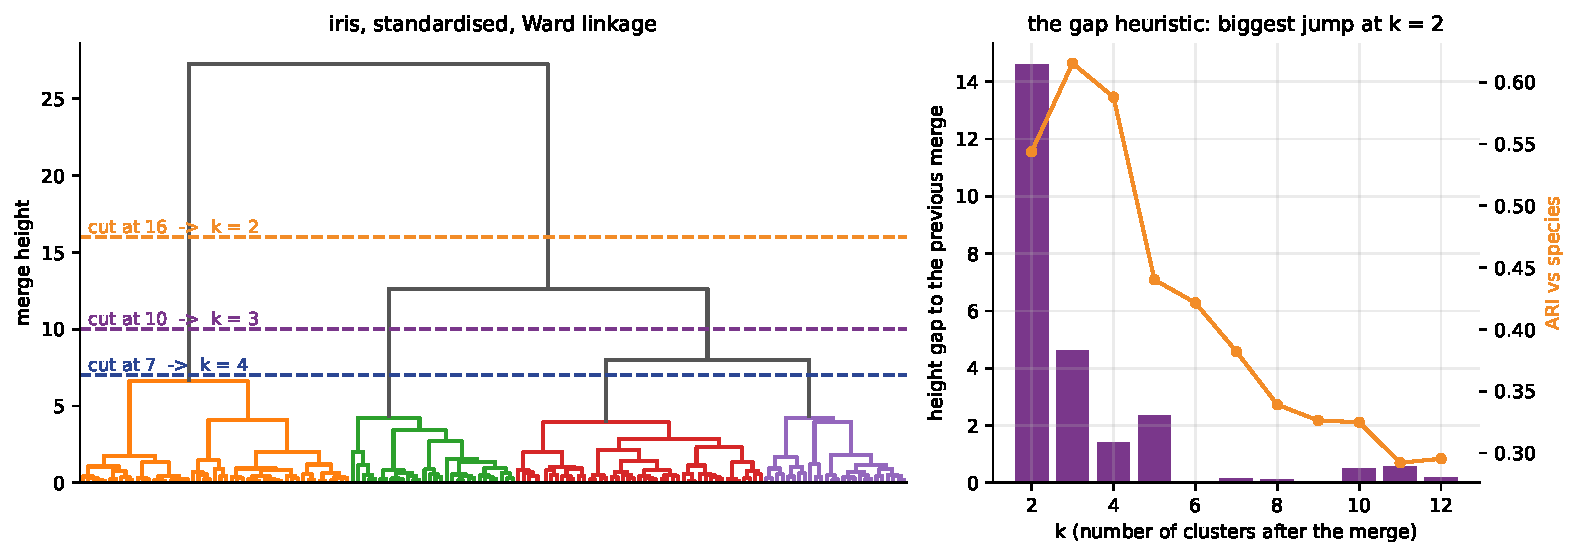
\includegraphics[width=\textwidth]{cutting.pdf}
  \caption{Left: the iris dendrogram under Ward linkage on standardised
    features, with three candidate cuts. Right: the height gap at each $k$
    (bars) against the ARI with the true species (orange line). The biggest
    gap is at $k=2$; the best agreement with the species is at $k=3$.}
  \label{fig:cutting}
\end{figure}

\subsection{What the $k=3$ cut actually did}

\begin{codeout}
k = 3 against the true species:
           cluster 1  cluster 2  cluster 3
species 0           49          1          0
species 1            0         27         23
species 2            0          2         48
\end{codeout}

Setosa is recovered almost exactly ($49$ of $50$). Versicolor and virginica
are split $27$/$23$ and $2$/$48$ --- the boundary between them is genuinely
fuzzy in the measurements, and no unsupervised method is going to find it.
Figure~\ref{fig:irispca} shows the same thing geometrically, along with what
single linkage does to the identical data: $100$/$49$/$1$, one giant cluster
and a stray point, exactly the failure mode of Section~\ref{sec:shape}.

\begin{figure}[htbp]
  \centering
  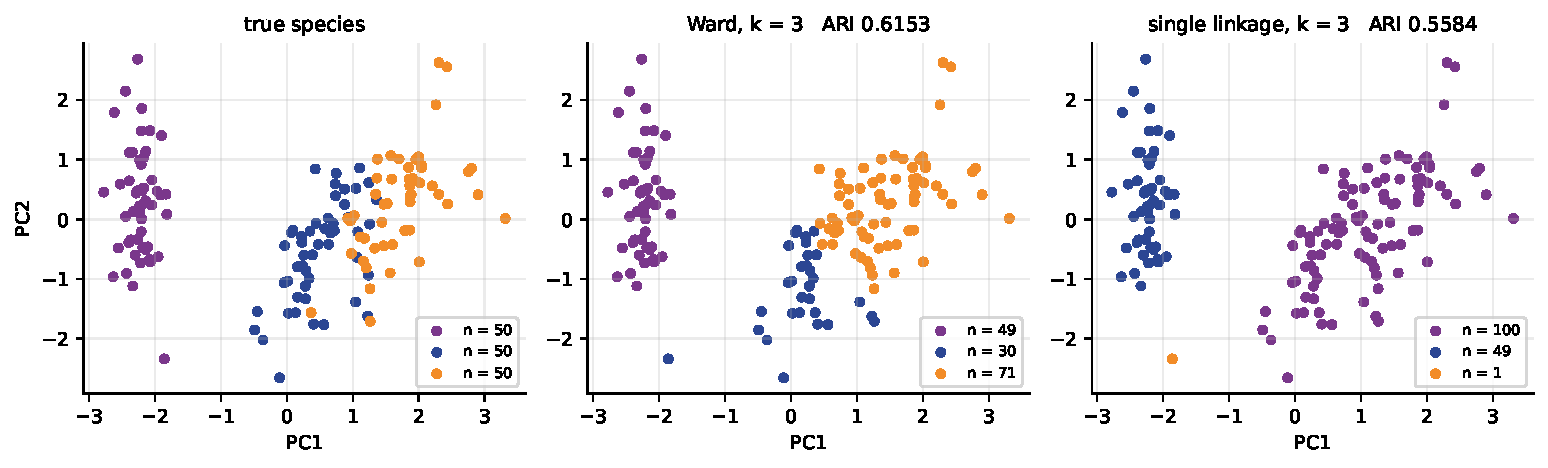
\includegraphics[width=\textwidth]{irispca.pdf}
  \caption{Iris in the first two principal components. Left: the true species.
    Centre: Ward at $k = 3$, ARI $0.6153$. Right: single linkage at $k = 3$,
    which peels off one point and one well-separated group and leaves the rest
    as one cluster of $100$.}
  \label{fig:irispca}
\end{figure}

\subsection{Two decisions that matter more than the linkage}

\textbf{Scaling.} The proximity matrix is computed from the raw columns, so
whichever column has the largest numbers dominates it.

\begin{codeout}
  raw centimetres  ARI at k=3 = 0.7312
  standardised     ARI at k=3 = 0.6153
  one column inflated 100x: ARI at k=3 = 0.2879
\end{codeout}

Note the direction: on iris, standardising made the answer \emph{worse}. The
four measurements are already in the same unit and the naturally larger
variance of the petal columns is genuine signal, which standardising throws
away. Inflating one column by $100$ destroys the result, as expected. The
lesson is not ``always standardise'' or ``never standardise'' --- it is that
this decision changes your clusters more than the choice of linkage does, so
make it deliberately and report it.

\textbf{The dissimilarity itself.} Average linkage accepts any proximity
matrix. Here are four on the wine data:

\begin{codeout}
  euclidean    average linkage, ARI -0.0054, sizes 3,174,1
  cityblock    average linkage, ARI 0.4730, sizes 51,126,1
  cosine       average linkage, ARI 0.7847, sizes 68,52,58
  correlation  average linkage, ARI 0.8224, sizes 56,58,64
\end{codeout}

An ARI of $-0.0054$ against $0.8224$, from the same linkage on the same rows.
Euclidean average linkage chains on this data and returns $3$/$174$/$1$;
correlation distance --- which asks whether two wines have the same
\emph{profile} across the thirteen measurements, ignoring overall magnitude
--- gets almost the right answer. Choose the dissimilarity by thinking about
what ``similar'' means for your objects. The previous lecture was about
exactly that, and this is where it pays.

\subsection{Is the tree faithful? The cophenetic correlation}

The \textbf{cophenetic distance} between two objects is the height of the node
where they first join. Comparing all $\binom{n}{2}$ cophenetic distances with
the original ones, by Pearson correlation, measures how much the tree
distorted the input.

\begin{lstlisting}
for m in ("single", "complete", "average", "centroid", "ward"):
    c, _ = cophenet(linkage(P6, method=m), pdist(P6))
    print("  %-9s cophenetic corr = %.4f" % (m, c))
\end{lstlisting}
\begin{codeout}
  single    cophenetic corr = 0.7152
  complete  cophenetic corr = 0.7370
  average   cophenetic corr = 0.7489
  centroid  cophenetic corr = 0.7480
  ward      cophenetic corr = 0.7372
\end{codeout}

Average linkage wins, which is no accident: it is the only one of the five
that is defined as a mean over all cross pairs, so it is the one built to
preserve average distances. A high cophenetic correlation says the tree is a
faithful summary of the matrix. It does \emph{not} say the clusters are
useful, and it should never be used on its own to choose a linkage --- if
faithfulness to the matrix were the goal, you would keep the matrix.

% =========================================================================
\section{Time and space}
\label{sec:cost}

\subsection{Space is the binding constraint}

HAC needs the proximity matrix. In condensed form that is $n(n-1)/2$
double-precision numbers.

\begin{codeout}
        n        pairs n(n-1)/2   condensed float64      full square
      100                4,950           38.7 KiB         78.1 KiB
    1,000              499,500            3.8 MiB          7.6 MiB
   10,000           49,995,000          381.4 MiB        762.9 MiB
   50,000        1,249,975,000            9.3 GiB         18.6 GiB
  100,000        4,999,950,000           37.3 GiB         74.5 GiB
1,000,000      499,999,500,000            3.6 TiB          7.3 TiB
measured: pdist on 10,000 points returns float64 of shape (49995000,) -> 381.4 MiB
\end{codeout}

\begin{keyidea}
At $n = 100{,}000$ the proximity matrix alone is $\mathbf{37.3}$\,\textbf{GiB}
--- and that is the compact triangular form, before the algorithm allocates
anything else. This one number is why hierarchical clustering does not appear
in production pipelines over large data, and no cleverness about the merge
loop can rescue it, because the memory is in the input, not the algorithm.
\end{keyidea}

Turn it around and ask what $n$ a machine can hold:

\begin{itemize}[leftmargin=*]
  \item $8$\,GiB of memory: $n < 46{,}341$.
  \item $64$\,GiB of memory: $n < 131{,}072$.
\end{itemize}

and even those assume nothing else is resident. Storing the matrix as
\texttt{float32} buys you a factor of $\sqrt{2}$ in $n$. It does not change
the shape of the problem.

\subsection{Time}

The naive algorithm --- rescan the whole matrix for the minimum at each of the
$n-1$ steps --- is $O(n^3)$: $O(n^2)$ per scan, $n$ scans. Good
implementations do better. SciPy uses a minimum-spanning-tree algorithm for
single linkage and the \textbf{nearest-neighbour chain} algorithm for
complete, average, weighted and Ward, both $O(n^2)$; the remaining methods,
including centroid and median, fall back to the naive $O(n^3)$ loop. All of
them use $O(n^2)$ memory.

\begin{codeout}
     n   pdist(s)  single(s)  complete(s)   ward(s)  centroid(s)  sklearn ward(s)
   250     0.0001     0.0004       0.0005    0.0005       0.0005          0.0011
   500     0.0003     0.0008       0.0027    0.0023       0.0019          0.0024
  1000     0.0021     0.0038       0.0091    0.0101       0.0107          0.0117
  2000     0.0060     0.0240       0.0453    0.0505       0.0567          0.0541
  4000     0.0230     0.1174       0.3034    0.2671       0.3053          0.2651
  8000     0.0857     0.4912       1.3648    1.2896       1.3383          1.2973
\end{codeout}
\begin{codeout}
  quantity        fitted exponent p in t = c * n^p
  pdist           2.00
  single          2.18
  complete        2.28
  ward            2.27
  centroid        2.31
  sklearn ward    2.11
\end{codeout}

Fitting $t = c\,n^p$ on the log-log line gives exponents near $2$, not $3$,
which is what the documentation promises. Centroid measures $2.31$ despite
being the naive $O(n^3)$ implementation --- at $n \le 8000$ the quadratic
matrix work still dominates its constant, and the cube has not yet taken over.
Report what you measure, not what the asymptotics say.

\begin{caution}[Timings are the one thing a seed cannot fix]
Every other number in these notes is reproducible: same data, same tree, same
heights on your machine as on mine. \textbf{The seconds in this section are
not.} They depend on your processor, your BLAS build, your SciPy version and
what else is running, and repeated runs on the same machine moved the fitted
exponents by several hundredths without a single line of code changing.

So read the table for its \emph{shape} --- Ward and complete cost roughly ten
times \texttt{pdist}, and every method grows like $n^2$ --- and never quote a
second as though it were a property of the algorithm. Where a claim has to be
defensible, count operations instead, as the next block does. A student who
reports different seconds is right.
\end{caution}

To see the cube, time the textbook loop itself:

\begin{codeout}
  n =  100  naive   0.0124 s   scipy  0.00021 s
  n =  200  naive   0.0853 s   scipy  0.00036 s
  n =  400  naive   0.7196 s   scipy  0.00074 s
  n =  800  naive   6.1881 s   scipy  0.00274 s
  fitted exponent for the naive loop: 3.00
\end{codeout}

Close to $3$, on the nose: every doubling of $n$ multiplies the time by eight.

The wall-clock ratio in that block is a measurement, so state the claim in
something exact instead. The naive loop rescans every surviving pair at each
of the $n-1$ steps, which is
\[
  \sum_{m=2}^{n}\binom{m}{2} = \binom{n+1}{3}
  \quad\text{comparisons, against the } \binom{n}{2}
  \text{ entries the matrix holds.}
\]

\begin{codeout}
       n  naive comparisons   matrix entries        ratio
     100            166,650            4,950        33.7x
     200          1,333,300           19,900        67.0x
     400         10,666,600           79,800       133.7x
     800         85,333,200          319,600       267.0x
    8000     85,333,332,000       31,996,000      2667.0x
\end{codeout}

The ratio is exactly $(n+1)/3$: at $n = 800$ the textbook loop does
$\mathbf{267}$ times as much work as simply reading the whole proximity matrix
once, and at $n = 8000$, $\mathbf{2667}$ times. No timer is involved, so that
factor is the same on your machine as on mine --- which is what makes it worth
quoting. Every linkage, naive or not, makes exactly $n-1$ merges.

\begin{figure}[htbp]
  \centering
  
\includegraphics[width=\textwidth]{cost.pdf}
  \caption{Left: measured \texttt{linkage} time against $n$ on log-log axes,
    with $n^2$ and $n^3$ reference slopes. Right: the size of the condensed
    proximity matrix. The red marker is $n = 100{,}000$ at $37.3$\,GiB.}
  \label{fig:cost}
\end{figure}

\subsection{What the alternative costs}

For scale, $k$-means on the same points --- $O(nkdi)$ time, $O(n)$ memory:

\begin{codeout}
  k-means, n = 8,000     0.051 s   (the data itself is 312.5 KiB)
  k-means, n = 50,000    0.206 s   (the data itself is 1.9 MiB)
  k-means, n = 200,000   0.406 s   (the data itself is 7.6 MiB)
\end{codeout}

$k$-means at $n = 200{,}000$ takes well under a second and needs $7.6$\,MiB.
Ward at $n = 8{,}000$ takes a little over a second and needs $244$\,MiB.

Again, the seconds are measurements; the reason behind them is not. Each Lloyd
iteration computes $nk$ distances --- $600{,}000$ at $n = 200{,}000$, $k = 3$
--- while HAC must compute all $n(n-1)/2 = 19{,}999{,}900{,}000$ before it can
make its first merge. That is a factor of $\mathbf{33{,}333}$, exactly, and it
is the real reason the second column of the table is flat and the first is
not. Extrapolating the measured $n^2$ behaviour, Ward at $n = 100{,}000$ would
need a few minutes of compute --- and $37.3$\,GiB of memory, which is the part
that actually stops you.

\begin{keyidea}
Hierarchical clustering is a small-$n$ method. Under a few thousand objects it
is comfortable, deterministic, and gives you the whole tree. Above about
$50{,}000$ it is simply unavailable. If you need a hierarchy over large data,
the standard route is to summarise first --- run $k$-means with a large $k$,
or use a method built for the purpose such as BIRCH --- and then run HAC on
the summaries.
\end{keyidea}

\begin{tryit}[Find your own ceiling]
Run \texttt{pdist} on $5{,}000$, $10{,}000$ and $20{,}000$ random points and
watch the memory. The expected sizes are $95.4$\,MiB, $381.4$\,MiB and
$1.5$\,GiB. Then compute where your machine gives out: solve
$n(n-1)/2 \times 8 = M$ for your available $M$. You will be surprised how
small the answer is.
\end{tryit}

% =========================================================================
\section{Agglomerative against divisive}
\label{sec:div}

Divisive clustering starts at the root and splits. The difficulty is at the
very first step. A cluster of $n$ objects has $2^{n-1} - 1$ non-trivial
two-way splits, and the agglomerative algorithm's first step only has
$\binom{n}{2}$ pairs to score.

\begin{codeout}
  n =  10   agglomerative first step:     45 pairs to score   divisive first step: 511 two-way splits
  n =  20   agglomerative first step:    190 pairs to score   divisive first step: 524,287 two-way splits
  n =  50   agglomerative first step:  1,225 pairs to score   divisive first step: 562,949,953,421,311 two-way splits
  n = 100   agglomerative first step:  4,950 pairs to score   divisive first step: 6.34e+29 two-way splits
\end{codeout}

At $n = 100$ that is $6.34 \times 10^{29}$ candidate splits for the first
decision alone. No exhaustive divisive method exists beyond toy sizes, so
practical divisive algorithms use a heuristic for the split --- DIANA
repeatedly moves the object with the largest average dissimilarity into a
splinter group; \emph{bisecting $k$-means} just runs $k$-means with $k=2$ and
recurses.

On six points the exhaustive search is affordable ($2^5 - 1 = 31$ splits), so
Figure~\ref{fig:updown} can show the real thing:

\begin{codeout}
  divisive step 1: {ABCDEF}  ->  {ABCD} | {EF}   SSE drop 36.333
  divisive step 2: {ABCD}    ->  {AB} | {CD}     SSE drop 10.000
  divisive step 3: {EF}      ->  {E} | {F}       SSE drop  8.000
  divisive step 4: {AB}      ->  {A} | {B}       SSE drop  2.500
  divisive step 5: {CD}      ->  {C} | {D}       SSE drop  0.500
\end{codeout}

The optimal top-down tree is \textbf{exactly the Ward agglomerative tree read
backwards}, and the first split's SSE drop, $36.333$, is the quantity
$\Delta(\{A,B,C,D\}, \{E,F\})$ computed by hand in Section~\ref{sec:linkage}.
That agreement is a happy accident of a small clean example; it is not
guaranteed and does not hold in general.

\begin{figure}[htbp]
  \centering
  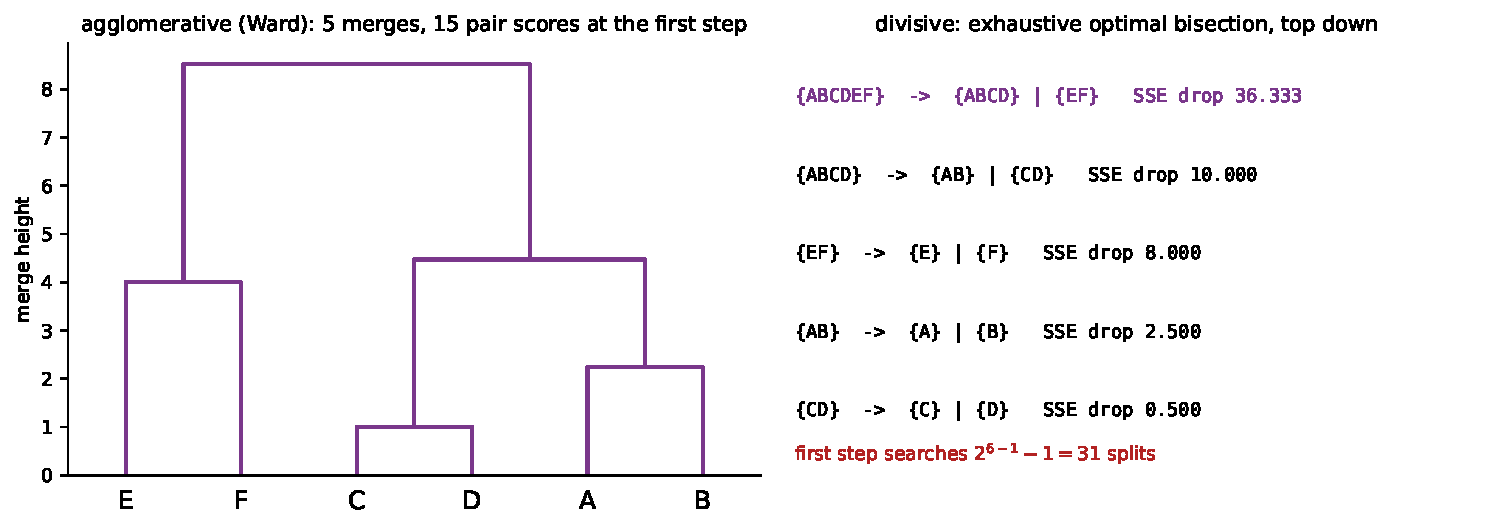
\includegraphics[width=\textwidth]{updown.pdf}
  \caption{The same six points, both directions. Left: Ward agglomerative,
    five merges, $15$ pair scores at the first step. Right: exhaustive optimal
    bisection, five splits, $31$ candidate splits at the first step --- and
    the identical tree.}
  \label{fig:updown}
\end{figure}

On real data with a heuristic split:

\begin{codeout}
  wine, 178 rows, standardised, k = 3
  agglomerative (Ward)         ARI 0.7899  sizes 56,64,58
  divisive (bisecting k-means) ARI 0.7062  sizes 51,62,65
  agreement between the two partitions: ARI 0.7757
  n =  1000  Ward HAC   0.009 s   bisecting k-means   0.004 s   ratio   2.1x
  n =  4000  Ward HAC   0.270 s   bisecting k-means   0.003 s   ratio  81.6x
  n =  8000  Ward HAC   1.313 s   bisecting k-means   0.005 s   ratio 260.3x
\end{codeout}

Comparable quality, and the divisive version is two orders of magnitude
faster at $n = 8000$ --- those seconds are a measurement on one machine, so
take the exact statement instead: Ward must compute all
$n(n-1)/2 = 31{,}996{,}000$ pairwise distances before its first merge, while
bisecting $k$-means never computes more than $nk$ at a time. It is also still
$O(n)$ in memory against Ward's $O(n^2)$. So why is agglomerative the
default?
Two reasons. It is \textbf{deterministic}, whereas bisecting $k$-means depends
on a random initialisation. And it gets the \textbf{bottom} of the tree right:
divisive methods make their coarsest decisions first, on the least
information, and a bad first split can never be repaired. If you care about
fine structure --- which small groups are most alike --- build bottom-up. If
you only care about the top few levels of a large data set, top-down is the
practical choice.

% =========================================================================
\section{Summary}
\label{sec:summary}

\begin{enumerate}[leftmargin=*]
  \item A hierarchical clustering is a \textbf{nested family} of partitions,
    one for every $k$, drawn as a dendrogram. Leaf positions mean nothing;
    node heights mean everything.
  \item \textbf{HAC} starts from $n$ singletons and merges the two closest
    clusters $n-1$ times. It is greedy, deterministic and irrevocable.
  \item Its only input is the \textbf{proximity matrix}, so it works on any
    dissimilarity --- except centroid and Ward, which need Euclidean points.
  \item \textbf{Single linkage} $= \min$ over cross pairs. Update: element-wise
    minimum. It chains.
  \item \textbf{Complete linkage} $= \max$. Update: element-wise maximum. Merge
    height $=$ cluster diameter. It makes compact clusters.
  \item On the six points these give completely different trees: heights
    $1,\ 2,\ 2.2361,\ 3.1623,\ 4$ against
    $1,\ 2.2361,\ 4,\ 4.4721,\ 8.6023$, and at $k=3$ the partitions
    $\{ABCD\}\{F\}\{E\}$ against $\{AB\}\{CD\}\{EF\}$.
  \item \textbf{Average} $=$ mean of all $n_A n_B$ cross distances.
    \textbf{Centroid} $= \lVert c_A - c_B\rVert$. \textbf{Ward} $=
    \sqrt{2 n_A n_B/(n_A{+}n_B)}\,\lVert c_A - c_B\rVert$, which is
    $\sqrt{2\Delta}$ for the within-cluster sum-of-squares increase $\Delta$.
  \item \textbf{Lance--Williams} unifies all five in one recurrence with four
    constants, which is why one implementation serves them all.
  \item Linkage encodes a belief about cluster shape. Single says
    ``connected'' --- ARI $1.000$ on two moons, ARI $0.000$ on three touching
    blobs. Complete and Ward say ``compact'' --- and cut long thin clusters
    across the middle.
  \item \textbf{Chaining}: twelve bridge points drop single linkage's fusion
    height from $5.571$ to $0.565$ and turn a $[60,60]$ answer into
    $[131,1]$. Complete and Ward do not move.
  \item \textbf{Centroid linkage can invert}: on three points, merges at
    $0.9675$ then $0.8683$. The dendrogram is then unreadable. Average
    linkage answers a similar question and is monotone.
  \item \textbf{Cut} by count or by height. The largest height gap is a
    heuristic and it tends to point at small $k$ --- on iris it says $2$
    where the species say $3$.
  \item \textbf{Scaling and the choice of dissimilarity} change the answer
    more than the linkage does: on wine, average linkage scores ARI
    $-0.0054$ with Euclidean distance and $0.8224$ with correlation distance.
  \item \textbf{Cost}: $O(n^2)$ space always; $O(n^2)$ time for good
    implementations and $O(n^3)$ for the naive loop, whose total work is
    exactly $\binom{n+1}{3}$ pair comparisons --- $(n+1)/3$ times the size of
    the matrix. At $n = 100{,}000$ the matrix is $37.3$\,GiB, which ends the
    discussion.
  \item \textbf{Divisive} clustering faces $2^{n-1}-1$ splits at the first
    step and is used only with a heuristic. Agglomerative is deterministic and
    gets the fine structure right.
\end{enumerate}

% =========================================================================
\section{Practice questions}
\label{sec:practice}

\begin{enumerate}[leftmargin=*, label=\textbf{Q\arabic*.}]
  \item \textbf{(By hand.)} Five objects have the proximity matrix
    \begin{center}\small
    \begin{tabular}{lrrrrr}
      \toprule
      & $P$ & $Q$ & $R$ & $S$ & $T$ \\
      \midrule
      $P$ & --  & 2 & 6 & 10 & 9 \\
      $Q$ & 2   & --& 5 & 9  & 8 \\
      $R$ & 6   & 5 & --& 4  & 5 \\
      $S$ & 10  & 9 & 4 & -- & 3 \\
      $T$ & 9   & 8 & 5 & 3  & -- \\
      \bottomrule
    \end{tabular}
    \end{center}
    Run \textbf{single linkage} to completion. Write out the proximity matrix
    after every merge, list the four merge heights, and draw the dendrogram.

  \item \textbf{(By hand.)} Run \textbf{complete linkage} on the same matrix,
    again writing out every intermediate matrix. Compare the two trees. At
    $k = 2$, do they agree?

  \item \textbf{(By hand.)} Run \textbf{average linkage} on the same
    five-object matrix, using the Lance--Williams average coefficients for
    every update and writing out the proximity matrix after every merge. List
    the four heights and compare them with Q1 and Q2. As a check on your first
    update, compute $d_{\text{single}}$, $d_{\text{complete}}$ and
    $d_{\text{average}}$ for $\{P,Q\}$ against $\{S,T\}$ directly from the
    four cross distances.

  \item Explain in three sentences why complete-linkage merge heights are
    never smaller than single-linkage merge heights on the same data at the
    same step, and why it is meaningless to compare a height of $4.0$ from a
    single-linkage tree with a height of $4.0$ from a complete-linkage tree.

  \item A colleague clusters $12{,}000$ customer records with Ward linkage
    and it works. They then
    try $150{,}000$ records on the same $16$\,GiB machine and it fails. Give
    the number that explains the failure, and state the largest $n$ that
    machine could handle if the matrix were the only thing in memory.

  \item Points $U = (0,0)$, $V = (1,0)$, $W = (0.45, 0.80)$. Run
    \textbf{centroid} linkage by hand: both merge heights. Is the dendrogram
    monotone? What is the general geometric reason?

  \item You cluster $2{,}000$ documents using a precomputed cosine
    dissimilarity matrix. Which of the five linkages may you use, and which
    must you not? Justify with one sentence per rejected method.

  \item Two clusters, $A$ with $3$ members and centroid $(0,0)$, and $B$ with
    $5$ members and centroid $(4,3)$. Compute the Ward merge cost $\Delta$ and
    the height SciPy would report. Then compute both again for $n_A = n_B = 4$
    with the same centroids, and say in one sentence what the comparison shows
    about Ward's preference for cluster sizes.

  \item Sketch a two-dimensional data set on which single linkage gives the
    right answer and Ward gives a badly wrong one, and a second data set where
    the reverse holds. For each, name the property of the data responsible.

  \item You have a dendrogram of $400$ genes. The merge heights near the top
    are $\ldots, 8.1,\ 8.4,\ 12.9,\ 21.6$. Where would the gap heuristic tell
    you to cut, what $k$ does that give, and what two checks should you run
    before believing it?
\end{enumerate}

% =========================================================================
\section{Solutions}
\label{sec:solutions}

\paragraph{Q1 --- single linkage, worked in full.}
The smallest entry in the matrix is $d(P,Q) = 2$.

\textbf{Step 1: merge $P$ and $Q$ at height 2.} The new row is the
element-wise minimum of the $P$ and $Q$ rows: $\min(6,5) = 5$ against $R$,
$\min(10,9) = 9$ against $S$, $\min(9,8) = 8$ against $T$.
\begin{center}\small
\begin{tabular}{lrrrr}
  \toprule
  & $R$ & $S$ & $T$ & $PQ$ \\
  \midrule
  $R$  & -- & 4 & 5 & 5 \\
  $S$  & 4  & --& \textbf{3} & 9 \\
  $T$  & 5  & \textbf{3} & --& 8 \\
  $PQ$ & 5  & 9 & 8 & -- \\
  \bottomrule
\end{tabular}
\end{center}

\textbf{Step 2: merge $S$ and $T$ at height 3.} New row $= \min$ of the $S$
and $T$ rows: $\min(4,5) = 4$ against $R$, $\min(9,8) = 8$ against $PQ$.
\begin{center}\small
\begin{tabular}{lrrr}
  \toprule
  & $R$ & $PQ$ & $ST$ \\
  \midrule
  $R$  & -- & 5 & \textbf{4} \\
  $PQ$ & 5  & --& 8 \\
  $ST$ & \textbf{4}  & 8 & -- \\
  \bottomrule
\end{tabular}
\end{center}

\textbf{Step 3: merge $R$ and $ST$ at height 4.} New row: $\min(5, 8) = 5$
against $PQ$.
\begin{center}\small
\begin{tabular}{lrr}
  \toprule
  & $PQ$ & $RST$ \\
  \midrule
  $PQ$  & -- & \textbf{5} \\
  $RST$ & \textbf{5}  & -- \\
  \bottomrule
\end{tabular}
\end{center}

\textbf{Step 4: merge at height 5.} Done.

Merge heights in order: $\mathbf{2,\ 3,\ 4,\ 5}$. The dendrogram: $P,Q$ join
at $2$; $S,T$ join at $3$; $R$ joins $\{S,T\}$ at $4$; the two groups join at
$5$. Monotone, as single linkage always is.

\paragraph{Q2 --- complete linkage on the same matrix.}
\textbf{Step 1: merge $P$ and $Q$ at 2}, new row $=$ element-wise maximum:
$\max(6,5) = 6$ against $R$, $\max(10,9) = 10$ against $S$, $\max(9,8) = 9$
against $T$.
\begin{center}\small
\begin{tabular}{lrrrr}
  \toprule
  & $R$ & $S$ & $T$ & $PQ$ \\
  \midrule
  $R$  & -- & 4 & 5 & 6 \\
  $S$  & 4  & --& \textbf{3} & 10 \\
  $T$  & 5  & \textbf{3} & --& 9 \\
  $PQ$ & 6  & 10 & 9 & -- \\
  \bottomrule
\end{tabular}
\end{center}
\textbf{Step 2: merge $S$ and $T$ at 3}, new row $= \max$: $\max(4,5) = 5$
against $R$, $\max(10,9) = 10$ against $PQ$.
\begin{center}\small
\begin{tabular}{lrrr}
  \toprule
  & $R$ & $PQ$ & $ST$ \\
  \midrule
  $R$  & -- & 6 & \textbf{5} \\
  $PQ$ & 6  & --& 10 \\
  $ST$ & \textbf{5}  & 10 & -- \\
  \bottomrule
\end{tabular}
\end{center}
\textbf{Step 3: merge $R$ and $ST$ at 5}, new row: $\max(6, 10) = 10$.
\begin{center}\small
\begin{tabular}{lrr}
  \toprule
  & $PQ$ & $RST$ \\
  \midrule
  $PQ$  & -- & \textbf{10} \\
  $RST$ & \textbf{10} & -- \\
  \bottomrule
\end{tabular}
\end{center}
\textbf{Step 4: merge at 10.} Heights: $2, 3, 5, 10$ against single linkage's
$2, 3, 4, 5$. Every complete height is $\ge$ the corresponding single height,
and the last is twice as large. The first two merges are identical because
both join singletons, where the linkage rule has nothing to choose between.

At $k = 2$ both give $\{P,Q\}$ and $\{R,S,T\}$: \textbf{they agree}. This
matrix is well behaved --- two tight groups with a clear gap --- and when the
data has genuine separated structure all reasonable linkages find it. The
linkage only matters when the structure is ambiguous, which is most of the
time.

\paragraph{Q3 --- average linkage, worked in full.}
\textbf{Step 1: merge $P$ and $Q$ at height 2.} Lance--Williams with
$n_P = n_Q = 1$ gives $\alpha_P = \alpha_Q = 1/2$, $\beta = \gamma = 0$, so the
new row is the element-wise \emph{mean}: $(6{+}5)/2 = 5.5$ against $R$,
$(10{+}9)/2 = 9.5$ against $S$, $(9{+}8)/2 = 8.5$ against $T$.
\begin{center}\small
\begin{tabular}{lrrrr}
  \toprule
  & $R$ & $S$ & $T$ & $PQ$ \\
  \midrule
  $R$  & -- & 4 & 5 & 5.5 \\
  $S$  & 4  & --& \textbf{3} & 9.5 \\
  $T$  & 5  & \textbf{3} & --& 8.5 \\
  $PQ$ & 5.5 & 9.5 & 8.5 & -- \\
  \bottomrule
\end{tabular}
\end{center}
\textbf{Step 2: merge $S$ and $T$ at height 3.} New row: $(4{+}5)/2 = 4.5$
against $R$, $(9.5{+}8.5)/2 = 9.0$ against $PQ$.
\begin{center}\small
\begin{tabular}{lrrr}
  \toprule
  & $R$ & $PQ$ & $ST$ \\
  \midrule
  $R$  & -- & 5.5 & \textbf{4.5} \\
  $PQ$ & 5.5 & --& 9.0 \\
  $ST$ & \textbf{4.5} & 9.0 & -- \\
  \bottomrule
\end{tabular}
\end{center}
\textbf{Step 3: merge $R$ and $ST$ at height 4.5.} Now the sizes differ, so
the coefficients are not $1/2$: $n_R = 1$, $n_{ST} = 2$, giving
$\alpha_R = 1/3$ and $\alpha_{ST} = 2/3$, so
\[
  d(RST, PQ) = \tfrac13(5.5) + \tfrac23(9.0)
             = 1.8333 + 6.0 = 7.8333 .
\]
\textbf{Step 4: merge at 7.8333.} Heights: $\mathbf{2,\ 3,\ 4.5,\ 7.8333}$,
which sit between single linkage's $2, 3, 4, 5$ and complete linkage's
$2, 3, 5, 10$ at every step --- as a mean between a minimum and a maximum
must.

\textbf{The check.} Cross pairs between $\{P,Q\}$ and $\{S,T\}$ are
$d(P,S) = 10$, $d(P,T) = 9$, $d(Q,S) = 9$, $d(Q,T) = 8$, so
\[
  d_{\text{single}} = 8, \qquad d_{\text{complete}} = 10, \qquad
  d_{\text{average}} = \frac{10+9+9+8}{4} = 9 ,
\]
and $9$ is exactly the $d(PQ, ST)$ the recurrence produced at step 2 without
revisiting any of the four original distances.

\paragraph{Q4 --- why complete $\ge$ single.}
Both are computed over the same finite set of cross distances
$\{d(a,b) : a \in A, b \in B\}$; the maximum of a non-empty set is never below
its minimum, so $d_{\text{complete}}(A,B) \ge d_{\text{single}}(A,B)$ for
every pair at every stage, and therefore the merge heights are ordered the
same way. Comparing $4.0$ from one tree with $4.0$ from the other is
meaningless because the two numbers answer different questions: one says
``there exists a pair this close'', the other says ``every pair is at least
this close''. They are the same units of length but not the same measurement,
in the same way that a minimum salary and a maximum salary are both in rupees
but are not comparable figures.

\paragraph{Q5 --- the memory failure.}
At $n = 150{,}000$ the condensed matrix holds $150000 \times 149999 / 2 =
11{,}249{,}925{,}000$ pairs at $8$ bytes each, which is $89{,}999{,}400{,}000$
bytes $\approx 83.8$\,GiB. The machine has $16$\,GiB. It fails during
\texttt{pdist}, before any clustering happens.

For the largest feasible $n$, solve $n(n-1)/2 \times 8 = 16 \times 2^{30}$,
i.e.\ $n^2 - n = 4 \times 2^{30} = 4{,}294{,}967{,}296$, giving
$n \approx 65{,}537$. In practice you would need headroom for the data, the
linkage matrix and the working arrays, so treat $n \approx 40{,}000$ as the
real ceiling on such a machine. At $12{,}000$ records the matrix is
$549$\,MiB, which is why the first run worked.

\paragraph{Q6 --- a centroid inversion.}
$d(U,V) = 1.0000$; $d(U,W) = \sqrt{0.45^2 + 0.80^2} = \sqrt{0.2025 + 0.64} =
\sqrt{0.8425} = 0.9179$; $d(V,W) = \sqrt{0.55^2 + 0.80^2} =
\sqrt{0.3025 + 0.64} = \sqrt{0.9425} = 0.9708$.

Smallest is $d(U,W) = 0.9179$: \textbf{first merge at $0.9179$}. Their
centroid is $c = (0.225, 0.400)$, and
\[
  \lVert c - V \rVert = \sqrt{(1 - 0.225)^2 + 0.400^2}
  = \sqrt{0.600625 + 0.16} = \sqrt{0.760625} = 0.8721 .
\]
\textbf{Second merge at $0.8721$}, which is below the first. Not monotone; the
drop is $0.0458$.

The general reason: the centroid of a merged pair lies strictly between its
two members, so it is closer to at least one outside point than one of the
members was. Averaging pulls inward, and centroid linkage measures from the
average.

\paragraph{Q7 --- which linkages on a cosine matrix.}
\textbf{Allowed}: single, complete and average. Each is defined purely as a
minimum, maximum or mean over entries of the given matrix, and never needs a
coordinate.

\textbf{Not allowed}: centroid, because $\lVert c_A - c_B \rVert$ requires
averaging the objects themselves and there is no meaningful centroid of a set
of documents in cosine space; and Ward, because its cost
$\frac{n_A n_B}{n_A+n_B}\lVert c_A - c_B\rVert^2$ is an increase in Euclidean
within-cluster variance and has no interpretation under a non-Euclidean
dissimilarity. SciPy will run both without complaint and return numbers that
mean nothing --- see the caution in Section~\ref{sec:linkage}.

\paragraph{Q8 --- two Ward costs.}
$\lVert c_A - c_B \rVert = \sqrt{4^2 + 3^2} = 5$, so
$\lVert c_A - c_B\rVert^2 = 25$.

With $n_A = 3$, $n_B = 5$: $\Delta = \frac{3 \times 5}{8} \times 25 =
\frac{15}{8} \times 25 = 46.875$, and the reported height is
$\sqrt{2 \times 46.875} = \sqrt{93.75} = 9.6825$.

With $n_A = n_B = 4$: $\Delta = \frac{16}{8} \times 25 = 50$, and the height
is $\sqrt{100} = 10.0000$.

The same centroid separation costs more when the two clusters are
\emph{balanced}: $\frac{n_A n_B}{n_A + n_B}$ is maximised at equal sizes.
Ward therefore prefers to merge a small cluster into a large one rather than
join two medium ones, which is one reason its clusters come out similar in
size at any given level --- the big merges are deferred to the top of the
tree.

\paragraph{Q9 --- two sketches.}
\emph{Single wins}: two long concentric arcs, or two parallel thin bands, with
a clear gap between them and no noise in the gap. The clusters are
\textbf{connected but not convex}, and their centroids may even coincide, so
every compact linkage cuts across them. This is the moons row of
Figure~\ref{fig:linkgrid}: single ARI $1.000$, Ward ARI $0.241$.

\emph{Ward wins}: three roughly spherical Gaussian blobs of similar size that
lightly overlap, plus a few outliers. The overlap gives single linkage a chain
from one blob to the next, and the outliers become its top-level clusters.
This is the blobs row: single ARI $0.000$ with sizes $298/1/1$, Ward ARI
$0.697$.

The two responsible properties are \textbf{non-convexity with a clean gap}
(favours single) and \textbf{convexity with contact or noise} (destroys
single).

\paragraph{Q10 --- reading the gaps.}
The gaps are $8.4 - 8.1 = 0.3$, then $12.9 - 8.4 = 4.5$, then
$21.6 - 12.9 = 8.7$. The largest gap is the last one, so the heuristic says
cut between $12.9$ and $21.6$, which leaves \textbf{$k = 2$} clusters. The
second-largest gap, $4.5$, would give $k = 3$.

Two checks before believing it. First, compute an internal validity measure
--- silhouette on the same data --- for $k = 2, 3, 4, \ldots$ and see whether
it agrees; if silhouette peaks somewhere else, the gap was an artefact of
heights growing towards the root. Second, look at the \textbf{cluster sizes}:
a ``two cluster'' answer of $399$ and $1$ is the outlier-peeling failure of
Section~\ref{sec:shape}, not a structure, and it should be rejected
immediately. A third check, if you have any external information --- known
gene families, a downstream classification task --- is worth more than either.

% =========================================================================
\section{References and further reading}
\label{sec:refs}

All links were checked on 24 August 2026. Free resources are marked
\textbf{[free]}.

\subsection*{Textbooks}

\begin{itemize}[leftmargin=*]
  \item Han, Kamber and Pei, \emph{Data Mining: Concepts and Techniques}, 3rd
    edition, Morgan Kaufmann, 2012. \textbf{The prescribed text for this
    lecture.} \S10.3 hierarchical methods --- \S10.3.1 is agglomerative
    versus divisive, AGNES and DIANA, and the dendrogram; \S10.3.2 is distance
    measures in algorithmic methods, which is Section~\ref{sec:linkage} here
    in the notation the examination uses; \S10.3.3 BIRCH and \S10.3.4
    Chameleon are the scalable successors mentioned in
    Section~\ref{sec:cost}. \S2.4 is the dissimilarity background.
  \item James, Witten, Hastie, Tibshirani and Taylor, \emph{An Introduction to
    Statistical Learning with Python}. \textbf{[free]} \S12.4.2 is this
    lecture at a gentler pace --- the dendrogram, the four linkage types in a
    single table, the ``choice of dissimilarity measure'' subsection with the
    correlation-distance example that Section~\ref{sec:cut} measures, and the
    honest ``practical issues'' subsection on scaling and on the fact that
    small changes to the data change the tree.
    \url{https://www.statlearning.com/}
  \item Manning, Raghavan and Sch\"utze, \emph{Introduction to Information
    Retrieval}, Cambridge University Press, 2008. \textbf{[free, full text
    online]} Chapter 17 is the clearest short treatment in print: \S17.1 HAC
    and the dendrogram, \S17.2 single-link and complete-link \emph{with the
    chaining and outlier-sensitivity figures}, \S17.2.1 the time complexity
    of HAC, \S17.3 group-average, \S17.4 centroid clustering \emph{including
    inversions}, \S17.6 divisive clustering.
    \url{https://nlp.stanford.edu/IR-book/html/htmledition/hierarchical-clustering-1.html}
  \item Hastie, Tibshirani and Friedman, \emph{The Elements of Statistical
    Learning}, 2e, Springer. \textbf{[free]} \S14.3.12 is agglomerative
    clustering, with the monotonicity discussion and the warning that a
    dendrogram should not be read as a description of the data unless the
    cophenetic correlation is high --- which is Section~\ref{sec:cut} here.
    \url{https://hastie.su.domains/ElemStatLearn/}
  \item Tan, Steinbach, Karpatne and Kumar, \emph{Introduction to Data
    Mining}. The cluster-analysis chapter is the standard source for the
    proximity-matrix-update presentation used in Section~\ref{sec:single}, and
    the authors' lecture slides are free.
    \url{https://www-users.cse.umn.edu/~kumar001/dmbook/index.php}
  \item M\"uller and Guido, \emph{Introduction to Machine Learning with
    Python}, O'Reilly, 2016. \S3.5.2 agglomerative clustering --- short,
    practical, with the \texttt{scipy} dendrogram recipe. Notebooks
    \textbf{[free]}:
    \url{https://github.com/amueller/introduction_to_ml_with_python}
\end{itemize}

\subsection*{Online courses}

\begin{sloppypar}
\begin{itemize}[leftmargin=*]
  \item \textbf{NPTEL, Introduction to Machine Learning} --- Prof.\ Balaraman
    Ravindran, IIT Madras; the reference course for the semester. The
    clustering week covers hierarchical clustering, the linkage criteria and
    the dendrogram in the notation used here. \textbf{[free]}
    \url{https://nptel.ac.in/courses/106106139}
  \item \textbf{NPTEL, Data Mining} --- Prof.\ Pabitra Mitra, IIT Kharagpur.
    Follows the Han--Kamber--Pei chapter structure, so its clustering weeks
    map onto \S10.3 directly. \textbf{[free]}
    \url{https://nptel.ac.in/courses/106105174}
  \item \textbf{NPTEL, Introduction to Machine Learning} --- Prof.\ Sudeshna
    Sarkar, IIT Kharagpur. A second treatment worked at the board, if the
    first does not land. \textbf{[free]}
    \url{https://nptel.ac.in/courses/106105152}
  \item \textbf{SWAYAM} --- the national portal hosting NPTEL, with
    certification cycles. \textbf{[free]} \url{https://swayam.gov.in/}
\end{itemize}
\end{sloppypar}

\subsection*{Videos}

\begin{itemize}[leftmargin=*]
  \item StatQuest with Josh Starmer, \emph{StatQuest: Hierarchical Clustering}
    --- the proximity matrix, the merge loop and the dendrogram drawn out step
    by step at a whiteboard, with the linkage choice made explicit. Watch this
    one first; it is the video companion to Sections~\ref{sec:single}
    and~\ref{sec:complete}. \textbf{[free]} \url{https://youtu.be/7xHsRkOdVwo}
  \item Victor Lavrenko, \emph{Hierarchical Clustering 3: single-link vs.\
    complete-link} --- exactly the comparison of Section~\ref{sec:complete},
    including the chaining picture, in about eight minutes.
    \textbf{[free]} \url{https://youtu.be/VMyXc3SiEqs}
  \item \emph{Lecture 59 --- Hierarchical Clustering $|$ Stanford University}
    --- from the Mining Massive Datasets course; the part on what happens to
    hierarchical clustering when the data does not fit in memory is the
    lecture-hall version of Section~\ref{sec:cost}. \textbf{[free]}
    \url{https://youtu.be/rg2cjfMsCk4}
  \item StatQuest with Josh Starmer, \emph{StatQuest: K-means clustering} ---
    watch this before the next lecture, and note how differently it answers
    the same question: one $k$, chosen in advance, and a random start.
    \textbf{[free]} \url{https://youtu.be/4b5d3muPQmA}
\end{itemize}

\subsection*{Documentation and interactive explainers}

\begin{itemize}[leftmargin=*]
  \item SciPy reference, \texttt{scipy.cluster.hierarchy.linkage} --- the
    definitive statement of what each \texttt{method} computes, with the
    update formulas, and the Notes section that gives the complexity claims
    quoted in Section~\ref{sec:cost}: $O(n^2)$ for single (minimum spanning
    tree) and for complete, average, weighted and Ward
    (nearest-neighbour chain), $O(n^3)$ for the rest, $O(n^2)$ memory for all.
    It also states plainly that centroid, median and Ward are correct only for
    Euclidean distances. \textbf{[free]}
    \url{https://docs.scipy.org/doc/scipy/reference/generated/scipy.cluster.hierarchy.linkage.html}
  \item SciPy reference, \texttt{scipy.cluster.hierarchy} --- the rest of the
    module: \texttt{dendrogram}, \texttt{fcluster}, \texttt{cut\_tree},
    \texttt{cophenet} and \texttt{inconsistent}. \textbf{[free]}
    \url{https://docs.scipy.org/doc/scipy/reference/cluster.hierarchy.html}
  \item scikit-learn user guide, \emph{2.3. Clustering} --- \S2.3.6 is
    hierarchical clustering, with the linkage comparison, the connectivity
    constraints this lecture does not cover, and the table of which algorithm
    scales to what. \textbf{[free]}
    \url{https://scikit-learn.org/stable/modules/clustering.html}
  \item scikit-learn example, \emph{Comparing different hierarchical linkage
    methods on toy datasets} --- Figure~\ref{fig:linkgrid} is this
    demonstration rebuilt with measured ARIs. \textbf{[free]}
    \url{https://scikit-learn.org/stable/auto_examples/cluster/plot_linkage_comparison.html}
  \item scikit-learn example, \emph{Plot Hierarchical Clustering Dendrogram}
    --- how to get a full tree out of \texttt{AgglomerativeClustering} with
    \texttt{distance\_threshold=0}, which is the recipe
    Section~\ref{sec:scipy} refers to. \textbf{[free]}
    \url{https://scikit-learn.org/stable/auto_examples/cluster/plot_agglomerative_dendrogram.html}
\end{itemize}

\subsection*{Articles}

\begin{itemize}[leftmargin=*]
  \item J.\ H.\ Ward Jr., ``Hierarchical Grouping to Optimize an Objective
    Function'', \emph{Journal of the American Statistical Association}
    \textbf{58}(301), 236--244, 1963. The paper that introduced
    equation~\eqref{eq:wardcost}. Worth reading for how carefully it separates
    the \emph{criterion} from the \emph{algorithm} --- a distinction later
    implementations lost, which is what the Murtagh and Legendre survey below
    is about. \url{https://doi.org/10.1080/01621459.1963.10500845}
  \item G.\ N.\ Lance and W.\ T.\ Williams, ``A General Theory of
    Classificatory Sorting Strategies: 1. Hierarchical Systems'', \emph{The
    Computer Journal} \textbf{9}(4), 373--380, 1967. Equation~\eqref{eq:lw}
    and the coefficient table of Section~\ref{sec:lw}, in the paper that first
    wrote them down. \url{https://doi.org/10.1093/comjnl/9.4.373}
  \item F.\ Murtagh and P.\ Legendre, ``Ward's Hierarchical Clustering
    Method: Clustering Criterion and Agglomerative Algorithm''. \textbf{[free
    preprint]} Why the same words, ``Ward's method'', name two different
    computations in different software packages, and which one is Ward's. Read
    this before you trust a Ward dendrogram produced by an unfamiliar tool.
    \url{https://arxiv.org/abs/1111.6285}
  \item R.\ Sibson, ``SLINK: An optimally efficient algorithm for the
    single-link cluster method'', \emph{The Computer Journal} \textbf{16}(1),
    30--34, 1973. The $O(n^2)$ time, $O(n)$ \emph{space} algorithm for single
    linkage --- the one exception to the memory argument of
    Section~\ref{sec:cost}, and the reason single linkage scales further than
    the others. \url{https://doi.org/10.1093/comjnl/16.1.30}
  \item D.\ M\"ullner, ``Modern hierarchical, agglomerative clustering
    algorithms'', 2011. \textbf{[free]} The nearest-neighbour-chain algorithm
    and the generic scheme that SciPy implements; this is the reference SciPy
    itself cites for its complexity claims.
    \url{https://arxiv.org/abs/1109.2378}
\end{itemize}

\notesources{\AMLUnitVIISources}

\end{document}
